\documentclass[xcolor=dvipsnames]{beamer}

\usetheme{Darmstadt}
\usefonttheme[onlylarge]{structurebold}
\setbeamerfont*{frametitle}{size=\normalsize,series=\bfseries}
\setbeamertemplate{navigation symbols}{}

\usepackage[english]{babel}
\usepackage[cp1250]{inputenc}
\usepackage{times}
\usepackage[T1]{fontenc}


\usepackage{graphicx,amsmath} % Add all your packages here
\usepackage{amsfonts}
%\usepackage{listings}


\usepackage{url}

\usepackage{tikz}
\usetikzlibrary{arrows}
\tikzstyle{block}=[draw opacity=0.7,line width=1.4cm]


% correct bad hyphenation here
\hyphenation{op-tical net-works semi-conduc-tor IEEEtran}


\title{Information Extraction using PDT Tools and Inductive Logic Programming}

\author[D�dek]
{Jan D�dek}

\institute[MFF UK]
{
Department of Software Engineering, Faculty of Mathematics and Physics, Charles University in Prague, Czech Republic
}

\date[�FAL 2011]
{Aplikace NLP, 31. 3. 2011, MFF UK, Praha}



\begin{document}

\begin{frame}
  \titlepage
\end{frame}

\begin{frame}{Outline}
  \tableofcontents
\end{frame}


\section{Information Extraction Problem}

\subsection{Information Extraction}

\begin{frame}{Information Extraction Task}
\begin{itemize}
	\item The Task of Information Extraction	
		\begin{itemize}
			\item Automatically \alert{find} the information you�re looking for.
			\item Pick out the \alert{most useful bits}.
			\item \alert{Present} it in preferred manner, at the right level of detail.
		\end{itemize}

%	\item Semantic Web
%		\begin{itemize}
%			\item Web as universal medium for the exchange of information.
%			\item Not only for humans but also for \alert{software agents}.
%			\item Main problem today: \alert{lack of semantic data on the Web}.
%		\end{itemize}	
%	\item Extraction of information for the Semantic Web
%		\begin{itemize}
%			\item Let's use information extraction to produce semantic data.
%		\end{itemize}
\end{itemize}
\end{frame}

\begin{frame}{``Axis'' of Information Extraction}
\begin{itemize}
	\item Information depth
		\begin{itemize}
			\item ``Document labeling''\\
						
{\ttfamily
\begin{tabular}{rl}
	The event started at & \alert{half pas six}.\\
	& \alert{$\nwarrow$time\_expression}
\end{tabular}
}
			\item Uniform representation (``Semantic interpretation'')
{\ttfamily
\begin{tabular}{rl}
	The event started at & \alert{half pas six}.\\
	& \alert{$\nwarrow$time\_expression=18:30}
\end{tabular}
}
		\end{itemize}
	\item Task complexity
		\begin{itemize}
			\item Entity recognition
{\ttfamily \footnotesize
\begin{tabular}{lcl}
	\alert{J. D�dek} & is a PhD student at the & \alert{Charles Univ.}\\
	\alert{$\nwarrow$Person}&&\alert{$\nwarrow$Organization}
\end{tabular}
}
			\item Relation extraction
{\ttfamily \footnotesize
\begin{tabular}{lcl}
	\alert{J. D�dek} & is a PhD student at the & \alert{Charles Univ.}\\
	\alert{$\nwarrow$Person}& \alert{$\longrightarrow$has\_affiliation$\rightarrow$} &\alert{$\nwarrow$Organization}
\end{tabular}
}
		\end{itemize}	
\end{itemize}
\end{frame}



\subsection{Example Tasks}
\frame{\tableofcontents[currentsubsection]}


\begin{frame}{Example of the web-page with a report of a fire department}
\begin{columns}
\column{\textwidth}
\includegraphics[height=0.9\vsize]{img/DedVoj_article}
\end{columns}
\end{frame}

\begin{frame}{Text of an Accident Report and Contained Information}
\centerline{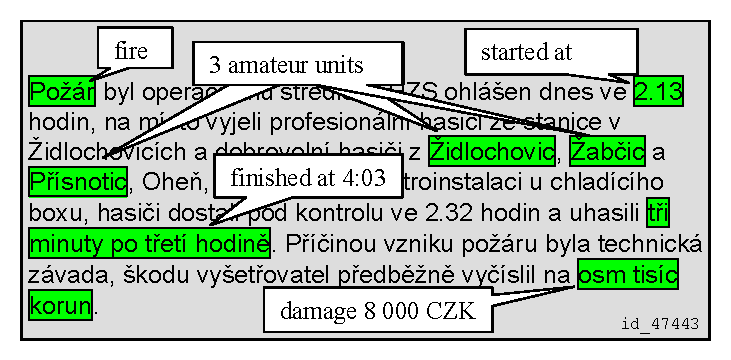
\includegraphics[height=0.5\vsize]{img/message}}
\bigskip
\begin{itemize}
	\item Information to be extracted is decorated.
%	\item See the last sentence on the \alert{next slide}.
\end{itemize}
\end{frame}



\begin{frame}{Acquisitions Corpus}
\begin{itemize}
	\item Corporate Acquisition Events
	\item Acquisitions v1.1 version\footnote{from the Dot.kom project's resources: \url{http://nlp.shef.ac.uk/dot.kom/resources.html}}
\end{itemize}
\centerline{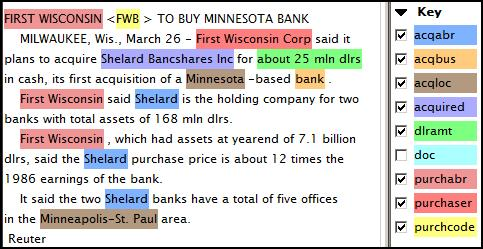
\includegraphics[width=0.7\hsize]{img/acquisitions}}
%\begin{itemize}
%	\item PROTON (PROTo ONtology) \url{http://proton.semanticweb.org/}
%\end{itemize}
\end{frame}




\section{Tools}
\frame{\tableofcontents[currentsection]}
\subsection{PDT}


\begin{frame}{Layers of linguistic annotation in PDT}
\begin{columns}
\column{.5\textwidth}
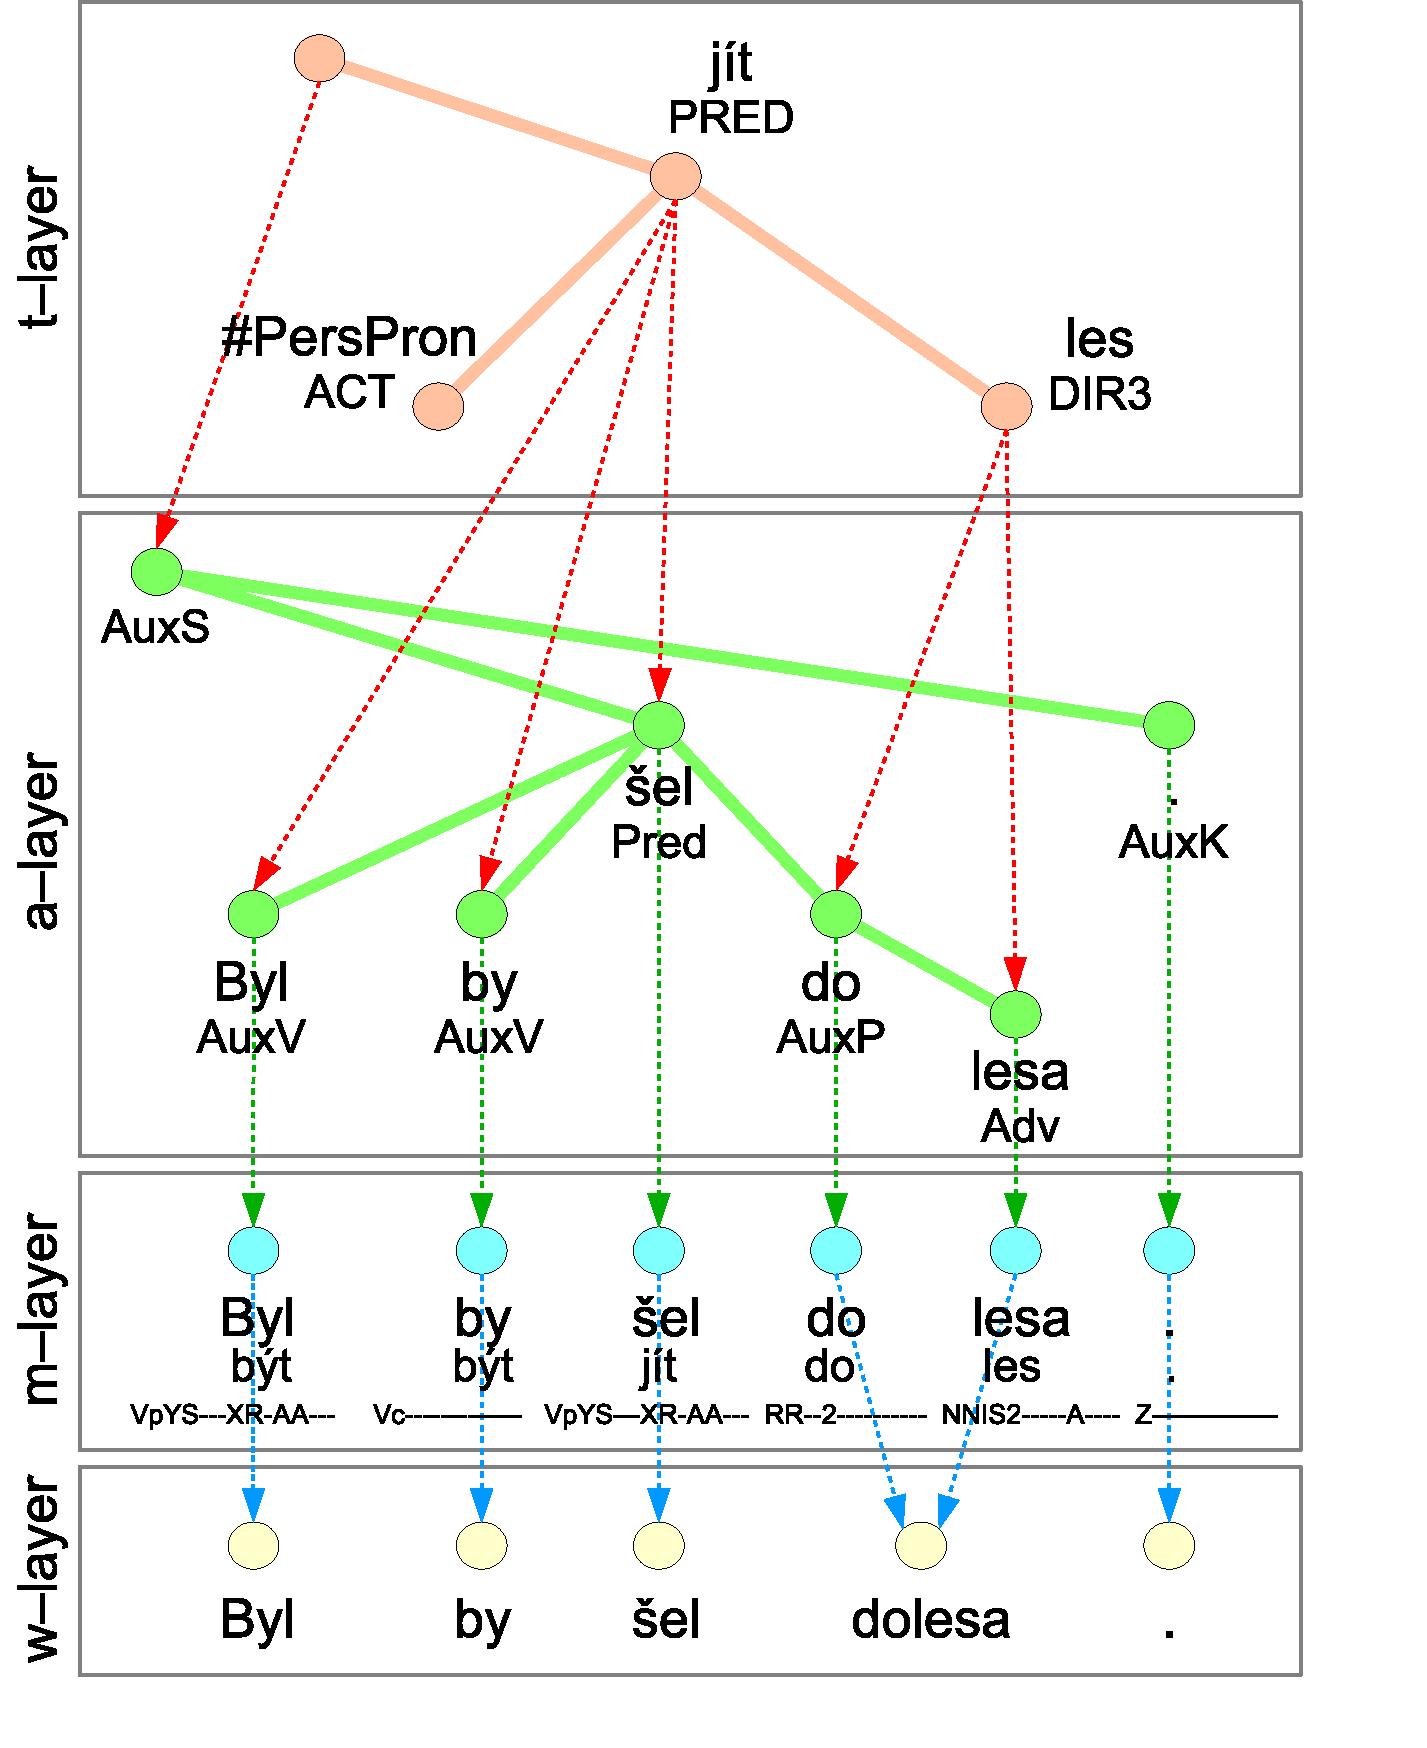
\includegraphics[height=0.9\vsize]{img/PDT_layers}
\column{.5\textwidth}
\begin{itemize}
	\item Tectogrammatical layer
	\item Analytical layer
	\item Morphological layer
\end{itemize}
\begin{itemize}
	\item PDT 2.0 on-line:\\\centerline{\scriptsize\url{http://ufal.mff.cuni.cz/pdt2.0/}} 
\end{itemize}
\vspace{2cm}
\emph{Sentence:}
\medskip
\\Byl by �el dolesa.
\\He-was would went toforest.
\end{columns}
\end{frame}

\begin{frame}{Tools for machine linguistic annotation}
	\begin{enumerate}
		\item Segmentation and tokenization
		\item Morphological analysis
		\item Morphological tagging	
		\item McDonnald's Maximum Spanning Tree parser\\ -- Czech adaptation
		\item Analytical function assignment
		\item Tectogrammatical analysis\\	-- Developed by V�clav Klime�
	\end{enumerate} 
	\begin{itemize}
		\item Available within the \alert{TectoMT}\footnote{\url{http://ufal.mff.cuni.cz/tectomt/}} project
	\end{itemize}
\end{frame}

%\begin{frame}{Example of a linguistic tree}
%\centerline{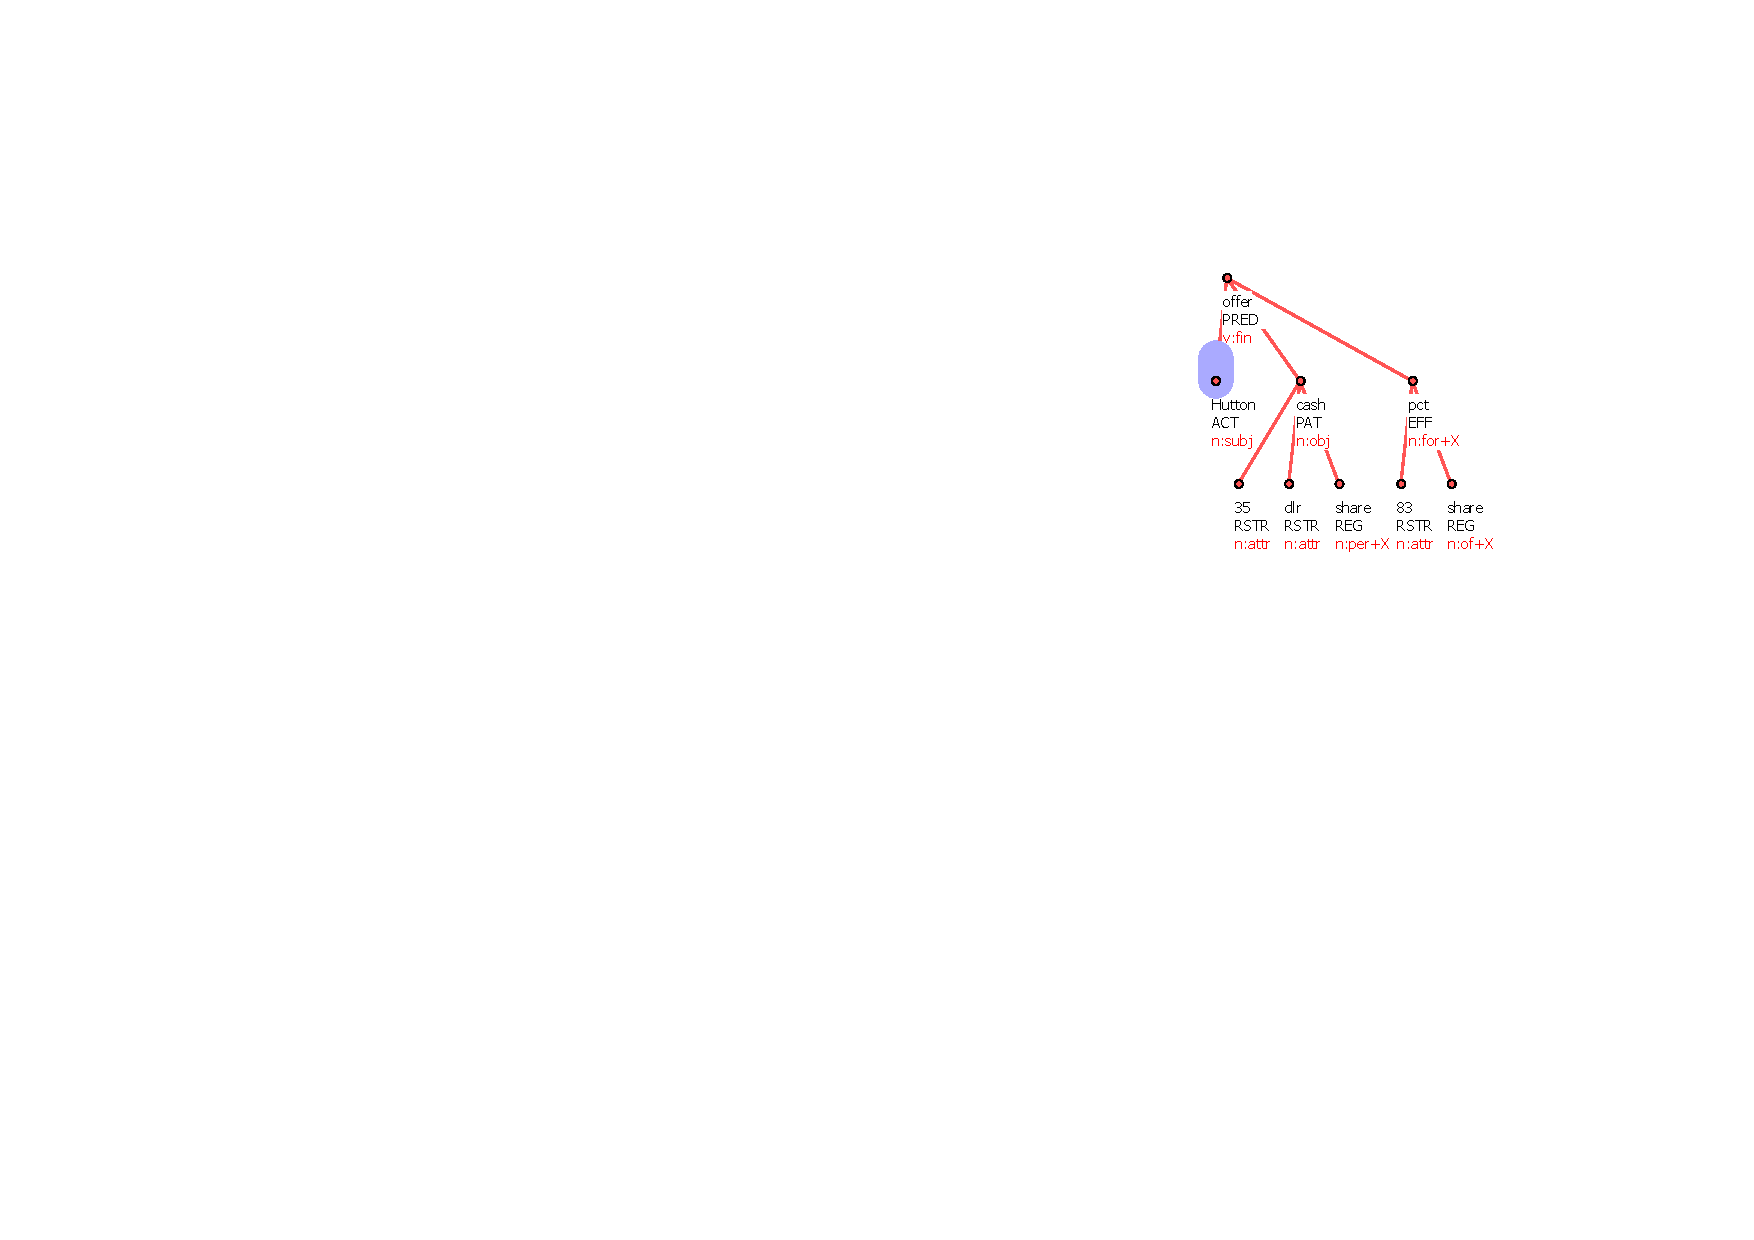
\includegraphics[height=0.7\vsize]{img/tree}}
%\begin{itemize}
%	\item Our IE method uses \alert{tree queries} (tree patterns)
%\end{itemize}
%\end{frame}


\begin{frame}{Example of an output tectogrammatical tree}
\begin{columns}
\column{.5\textwidth}
\includegraphics[height=0.9\vsize]{img/DedVoj_tecto_tree}
\column{.5\textwidth}
\begin{itemize}
	\item Lemmas
	\item Functors
	\item Semantic parts of speech
\end{itemize}
\vspace{0.7cm}
\emph{Sentence:}
\medskip
{\small
\\Ve zdemolovan�m trabantu na m�st� zem�eli dva mu�i -- 82let� senior a dal�� mu�, jeho� toto�nost zji��uj� policist�.
\medskip
\\Two men died on the spot in demolished trabant -- \dots }
\end{columns}
\end{frame}


\begin{frame}{Netgraph}
\begin{itemize}
	\item \url{http://quest.ms.mff.cuni.cz/netgraph/}
	\bigskip
	\item PML Tree Query 
	\item Query Engine and Query Language for TreeBanks
	\item \url{http://ufal.mff.cuni.cz/~pajas/pmltq/}
\end{itemize}
\end{frame}


\subsection{GATE}
\begin{frame}{GATE info}
\centerline{\includegraphics[height=0.1\vsize]{img/logo-gate}}
\bigskip
\begin{itemize}
	\item General Architecture for Text Engineering
	\item University of Sheffield, UK
\medskip	
	\item Natural Language Processing (NLP)
	\item Information Extraction (IE)
	\item Text Annotation
\medskip	
	\item Developed in \alert{Java}
\medskip	
	\item \url{http://gate.ac.uk/}
\end{itemize}
\end{frame}

\begin{frame}{GATE features}
\begin{itemize}
	\item Document and annotation management
	\item Language and processing utility resources	
\begin{itemize}
	\item Taggers, Parsers, Coreference-processors, Named entity recognizers, Alignment tools, WordNet, Yahoo search, etc
\end{itemize}
	\item JAPE grammar rules
	\item Performance evaluation tools
	\item Machine learning facilities
	\item Ontology support
\end{itemize}
\end{frame}

\begin{frame}{GATE screen shot}
\centerline{\includegraphics[height=0.9\vsize]{img/gatescreenshot}}
\end{frame}

\subsection{PDT in GATE}

\begin{frame}{Integration of PDT in GATE}
\begin{itemize}
%	\item GATE: General Architecture for Text Engineering
%	\item The University of Sheffield
%	\item \url{http://gate.ac.uk/}
%	\medskip
	\item Implemented \alert{Batch TectoMT Language Analyzer}	
	\begin{itemize}
		\item Transformation of PDT annotations to GATE
	\end{itemize}
	\medskip
	\item \alert{Netgraph} used as a tree viewer
	\begin{itemize}
		\item Works also for Standford Depndencies 
	\end{itemize}
\medskip	
	\item \url{http://czsem.berlios.de/}
\end{itemize}
\end{frame}


\begin{frame}{PDT in GATE}
\centerline{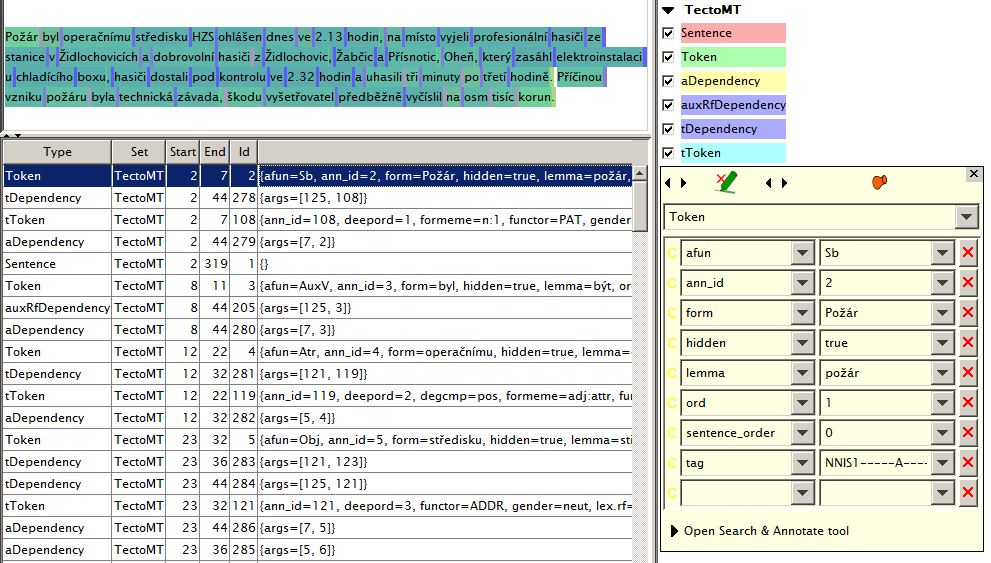
\includegraphics[width=1.16\hsize]{img/PDT_GATE}}
\end{frame}


\begin{frame}{Netgraph Tree Viewer in GATE (for Stanford Dependencies)}
\centerline{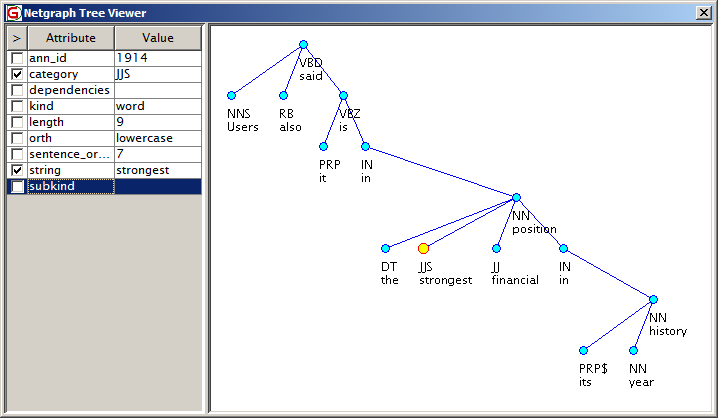
\includegraphics[width=\hsize]{img/netgraph_stanford}}
Sentence: Users also said it is in the strongest financial position in its 24-year history.
\end{frame}


\section{Our Solution}
\frame{\tableofcontents[currentsection]}

\subsection{Basic Idea}

\begin{frame}{How to extract the information about the damage of the accident?}
\centerline{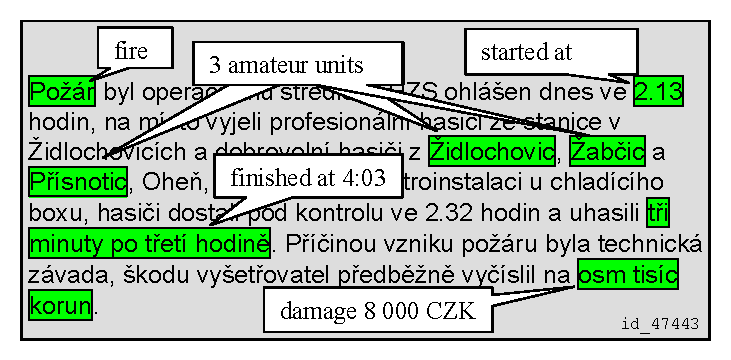
\includegraphics[height=0.5\vsize]{img/message}}
\bigskip
\begin{itemize}
	\item How to extract the information about the damage of the accident?
	\item See the last sentence on the \alert{next slide}.
\end{itemize}
\end{frame}

\begin{frame}{Corresponding linguistic tree}
\centerline{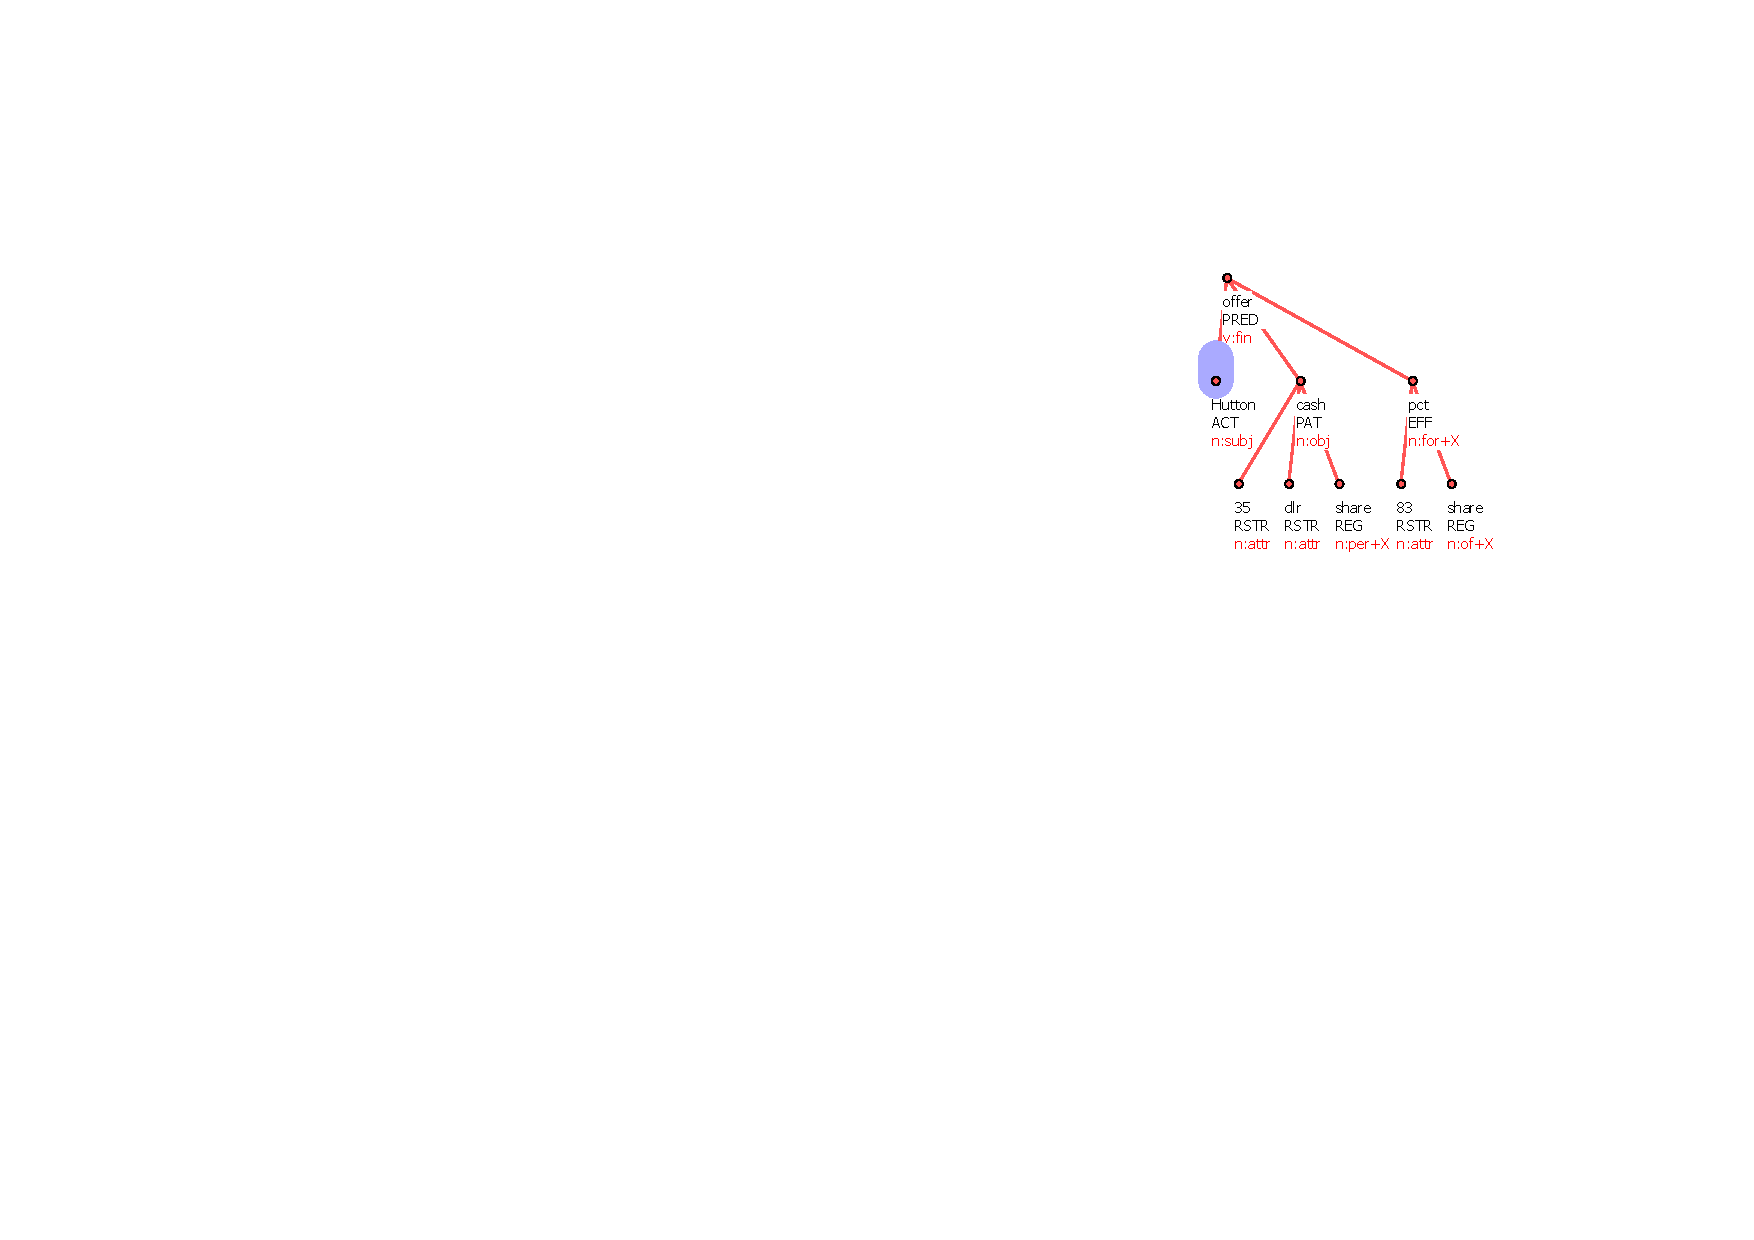
\includegraphics[height=0.7\vsize]{img/tree}}
\begin{itemize}
	\item Basic Idea: use \alert{tree queries} (tree patterns) to extract the information.
\end{itemize}
\end{frame}



\begin{frame}{Introduction of Our Solution}
\begin{itemize}
	\item Extraction of semantic information from texts.	
%		\begin{itemize}
%			\item In Czech language.
%			\item Coming from web pages.
%		\end{itemize}
%	\item Using of Semantic Web \alert{ontologies}.
%		\begin{itemize}
%			\item RDF, OWL
%		\end{itemize}
	\item Exploiting of linguistic tools.
		\begin{itemize}
			\item Mainly ``from'' the \alert{Prague Dependency Treebank} project.			
			\begin{itemize}
				\item Related tools -- language analyzers (TectoMT), Netgraph, etc.
			\end{itemize}
			\item Experiments with the Czech WordNet.
		\end{itemize}
\medskip	
	\item \alert{Rule based} extraction method.
		\begin{itemize}
			\item Extraction rules $\approx$ \alert{tree queries}
			\item ILP \alert{learning} of extraction rules
		\end{itemize}
\end{itemize}
\end{frame}

\begin{frame}{Schema of the extraction process}
\begin{columns}
\column{.3\textwidth}
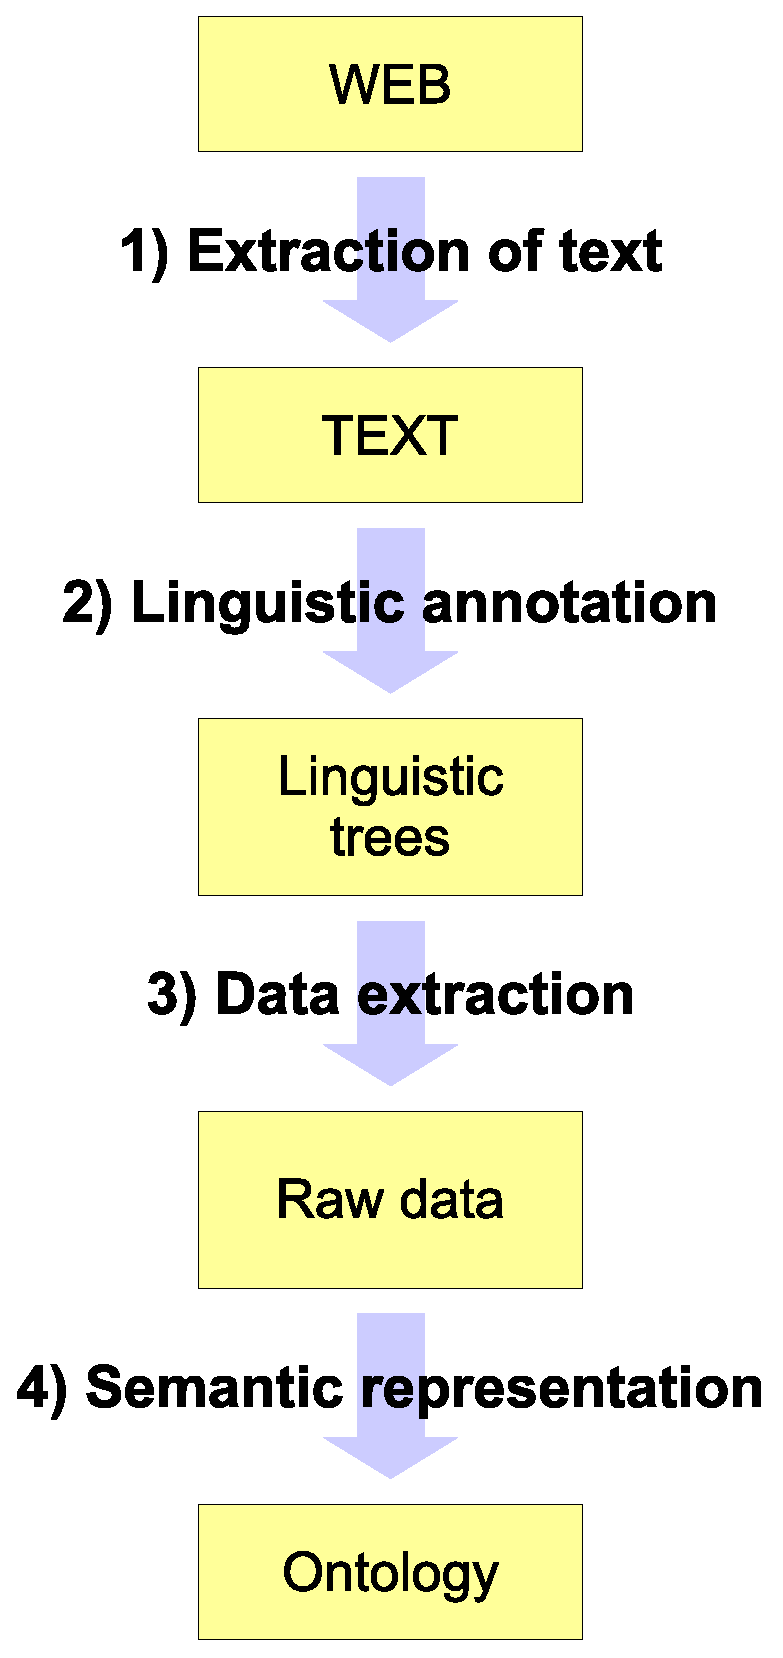
\includegraphics[height=0.8\vsize]{img/AP_schema1_en}
\column{.7\textwidth}
\begin{enumerate}
\item Extraction of text
\begin{itemize}
	\item Using \alert{RSS feed} to download pages.
	\item \alert{Regular expression} to extract text.
\end{itemize}
\item Linguistic annotation
\begin{itemize}
	\item Using \alert{chain} of 6 linguistic tools\\(see on next slides).
\end{itemize}
%In this phase the linguistic annotators process the extracted text and produce corresponding set of dependency trees representing the deep syntactic structure of individual sentences. We have used the linguistic tools described in the section~\ref{sec:ling_tools} for this task.
\item Data extraction
\begin{itemize}
	\item Exploitation of linguistic trees.
	\item Using \alert{extraction rules}.	
\end{itemize}
%We use the structure of tectogrammatic (i.e. deep syntactic) dependency trees to extract relevant data. 
\item Semantic representation of data
\begin{itemize}
	\item Ontology needed.
	\item Semantic interpretation of rules.
	\item Far from finished in current state.
\end{itemize}
%This phase consists of quite simple data transformation or conversion to the desired ontology format. But it is quite important to choose suitable ontology that will properly represent semantics of the data. We have not implemented this phase yet.
\end{enumerate}
\end{columns}
\end{frame}





\subsection{Manually Created Rules}
\frame{\tableofcontents[currentsubsection]}

\begin{frame}[plain]
\begin{columns}
\column{.67\textwidth}
%\centerline{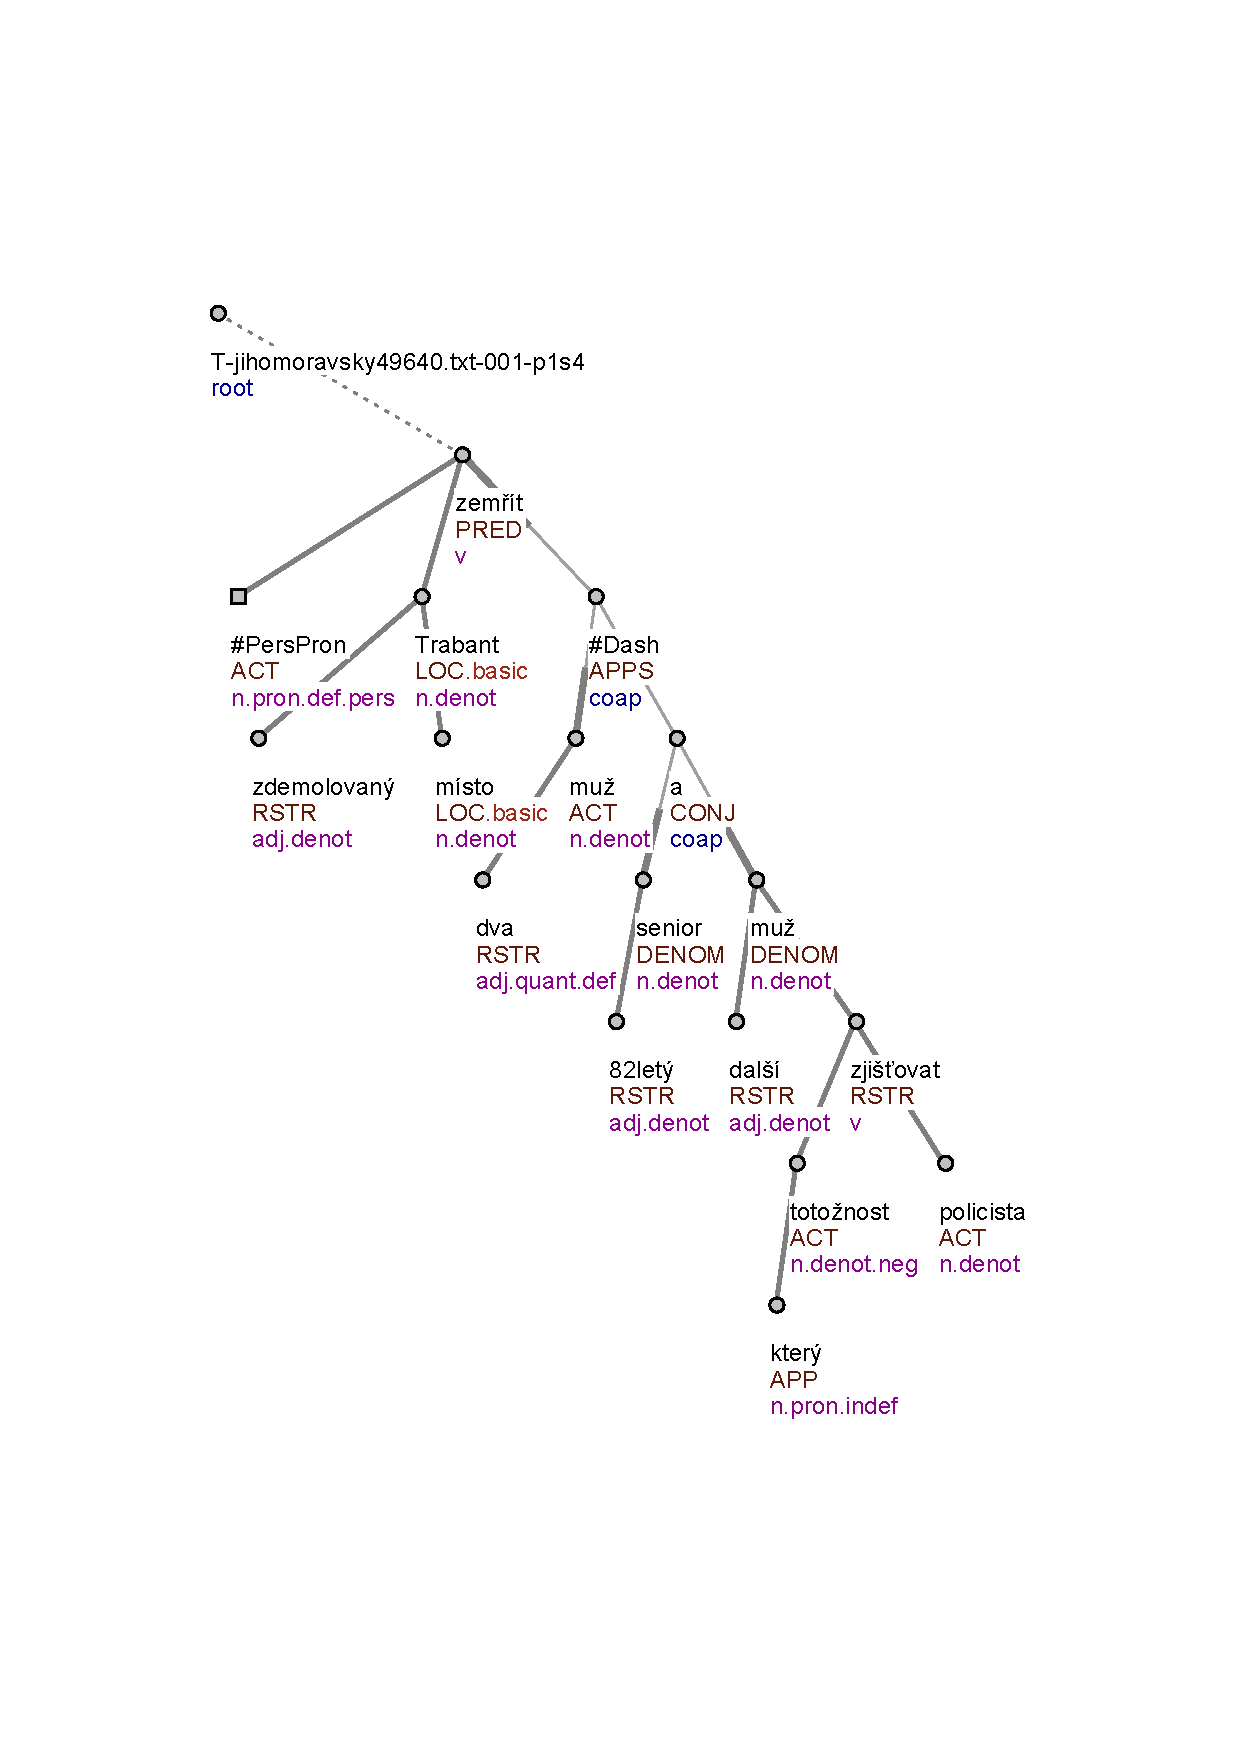
\includegraphics[height=1.1\vsize,width=\hsize]{img/TectogramaticalTree}}
\centerline{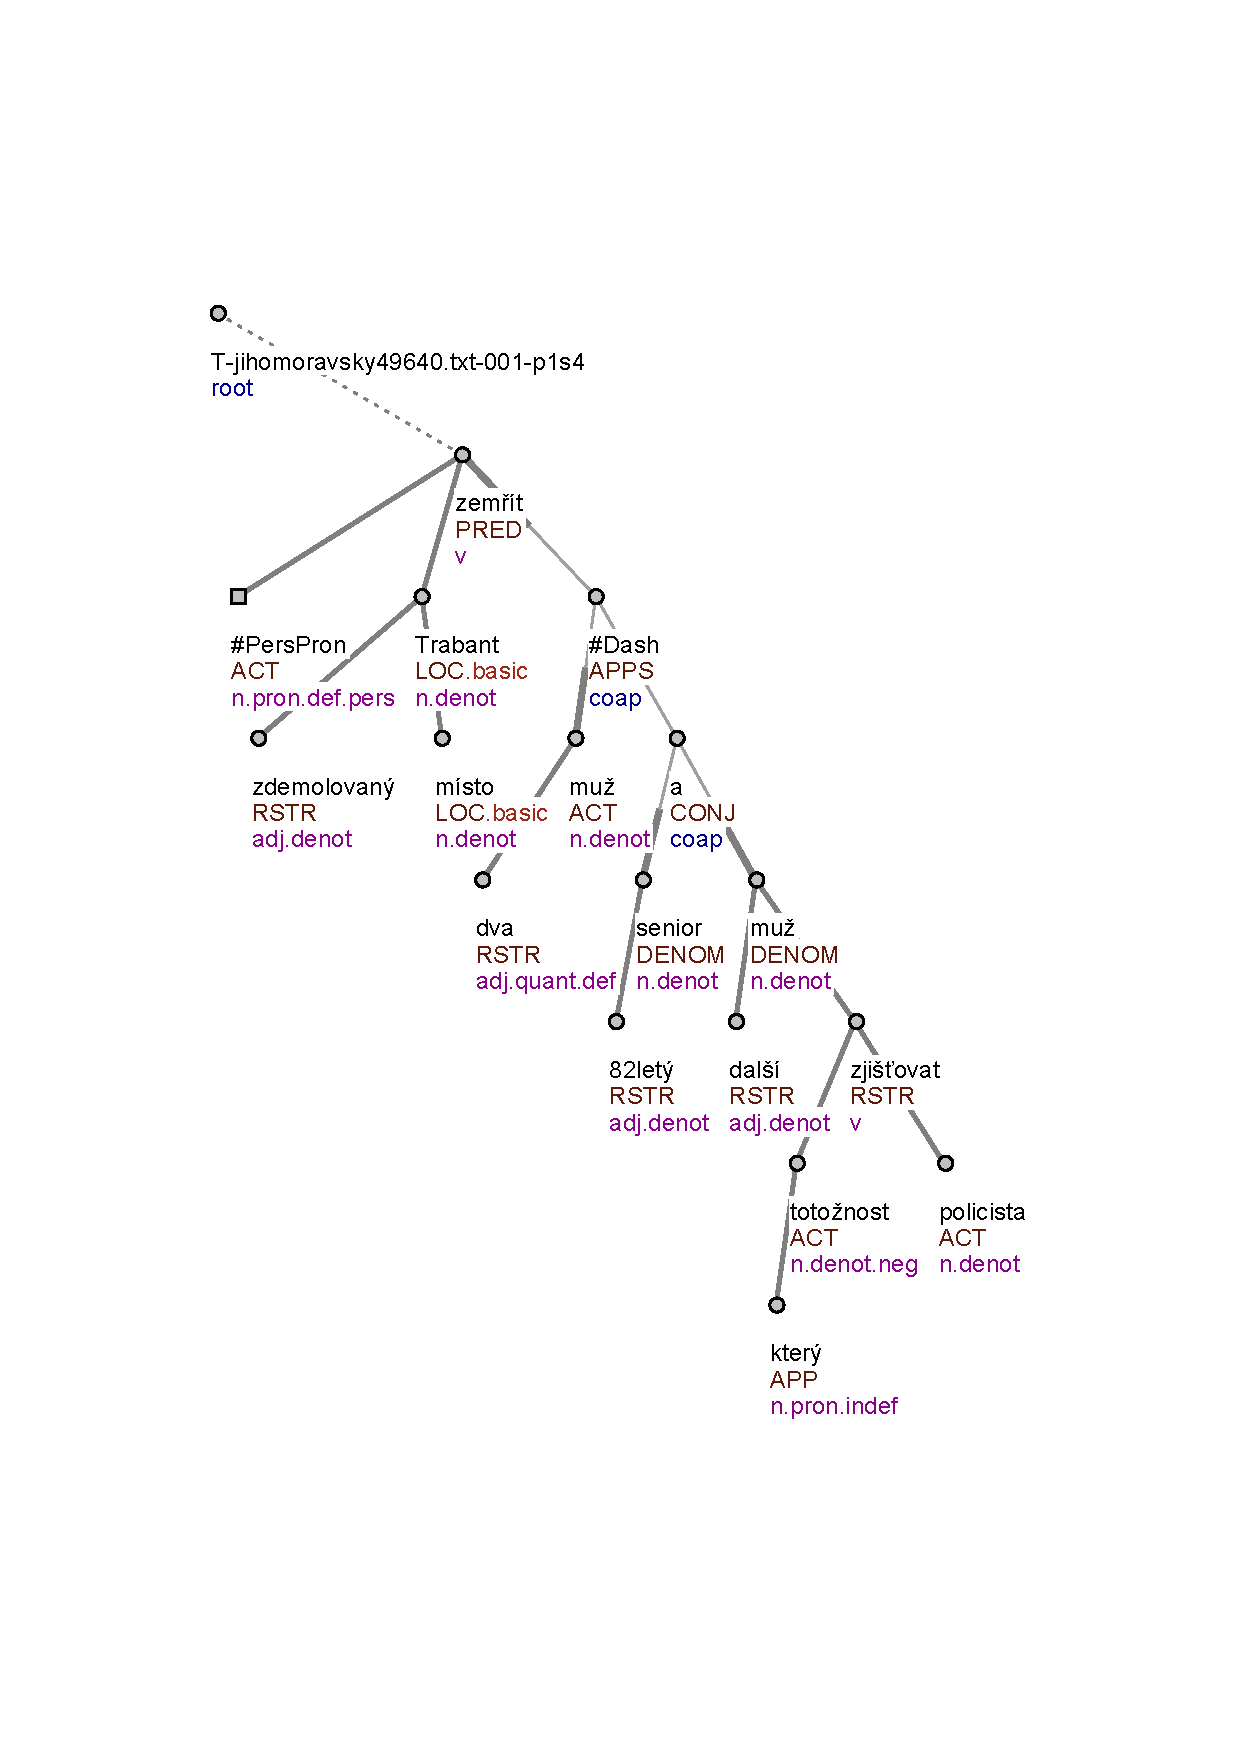
\includegraphics[height=1.1\vsize]{img/TectogramaticalTree}}
\column{.33\textwidth}
\begin{itemize}
	\item How to extract the information about \alert{two dead} people?
\end{itemize}
\vspace{2cm}
\end{columns}
\end{frame}



\begin{frame}{Extraction rules -- Netgraph queries}
\begin{center}
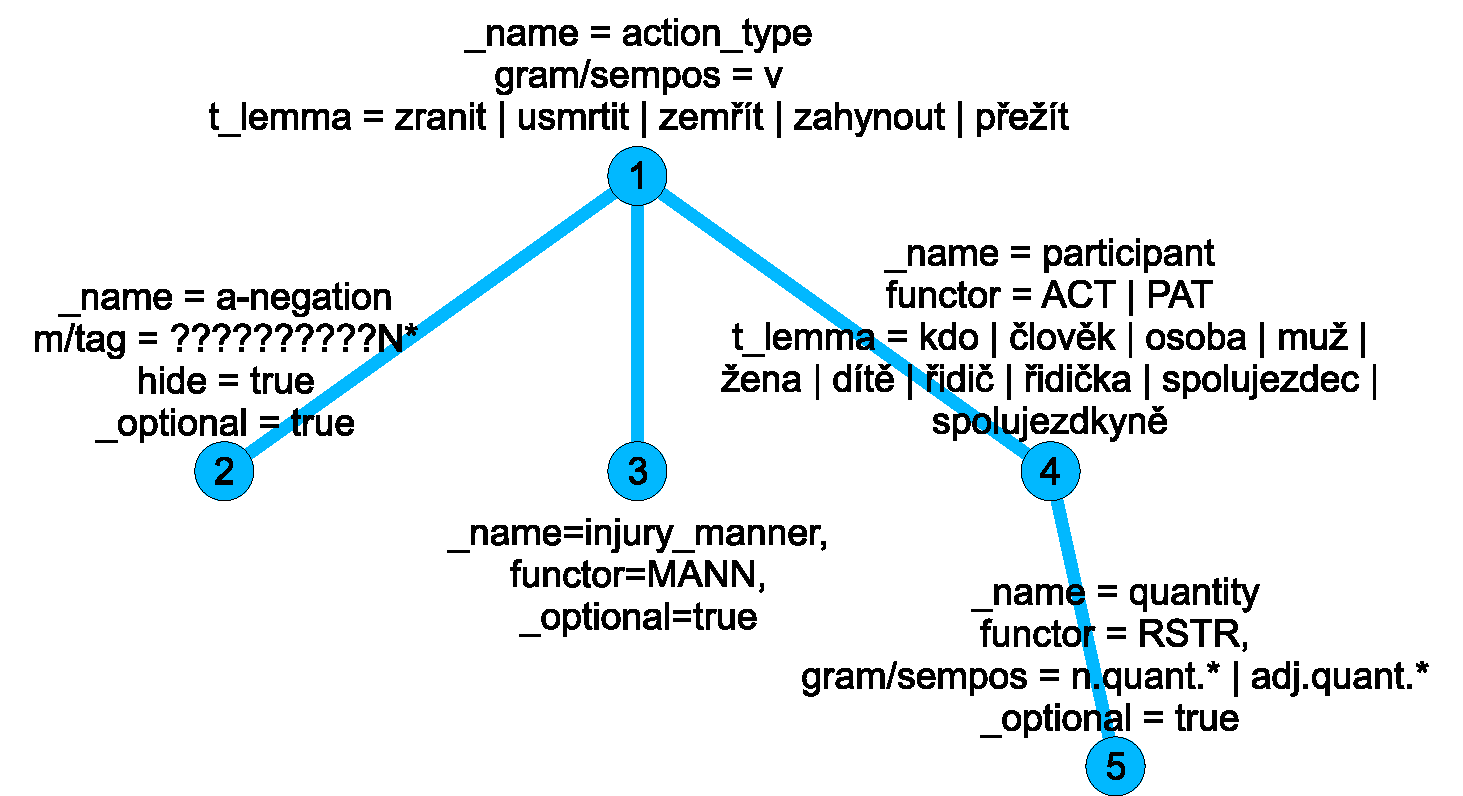
\includegraphics[height=0.6\vsize]{img/extract_patern}
\end{center}
\begin{itemize}
	\item Tree patterns on \alert{shape} and \alert{nodes} (on node attributes).
	\item Evaluation gives \alert{actual matches} of particular nodes.
	\item \alert{Names} of nodes allow use of references.
\end{itemize}
\end{frame}


\begin{frame}{Raw data extraction output}
%\begin{center}
\centerline{\includegraphics[height=0.8\vsize]{img/DedVoj_OutputQueryMatches}}
%\end{center}

{\scriptsize
\textbf{SELECT} \alert{action\_type}.t\_lemma, \alert{a-negation}.m\/tag, 
\alert{injury\_manner}.t\_lemma, \alert{participant}.t\_lemma,
\alert{quantity}.t\_lemma \textbf{FROM} \emph{***extraction rule***} 
}
\end{frame}

\begin{frame}{Extraction rules -- Environment Protection Use Case}
\begin{center}
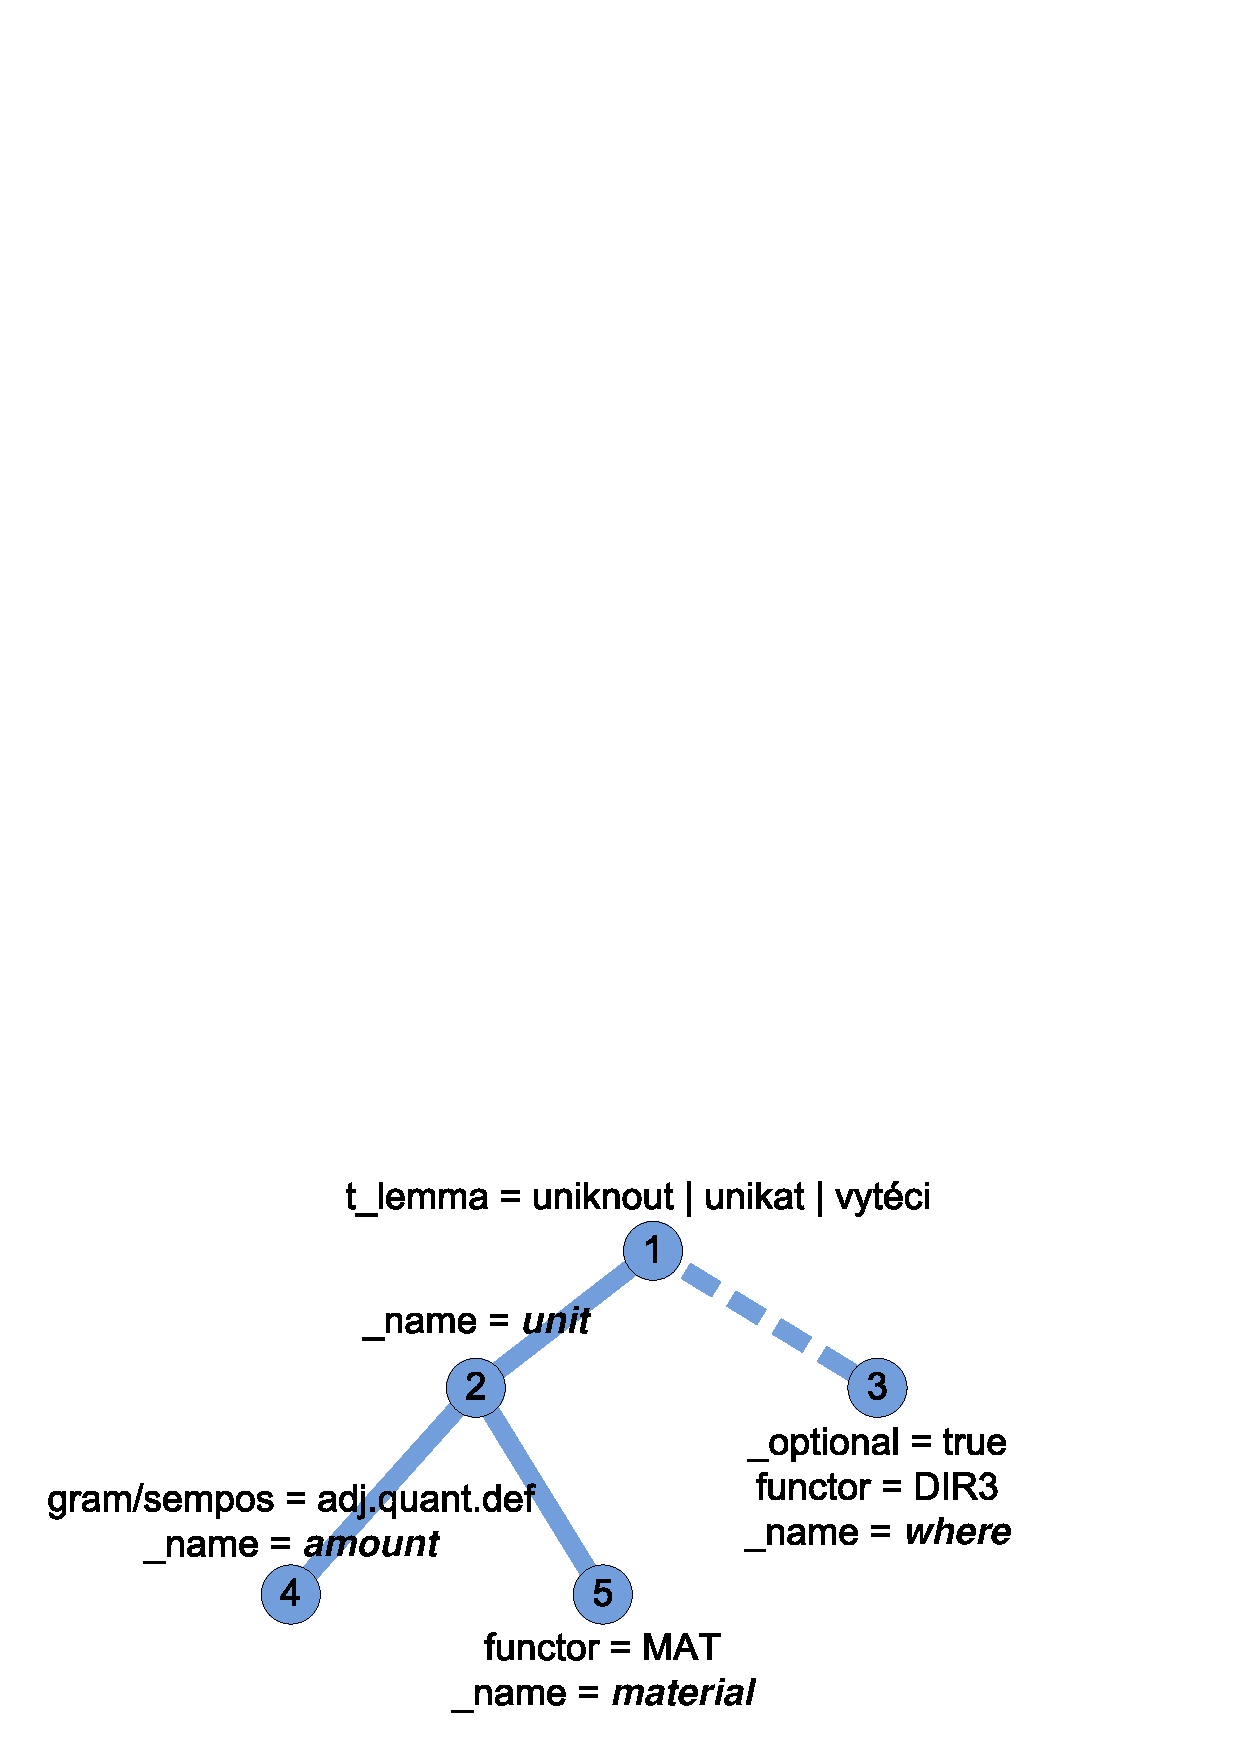
\includegraphics[height=0.6\vsize]{img/eenv_extr_rule}
\end{center}
%\begin{itemize}
%	\item Tree patterns on \alert{shape} and \alert{nodes} (on node attributes).
%	\item Evaluation gives \alert{actual matches} of particular nodes.
%	\item \alert{Names} of nodes allow use of references.
%\end{itemize}
\end{frame}



\begin{frame}{Matching Tree}
%\begin{center}
\centerline{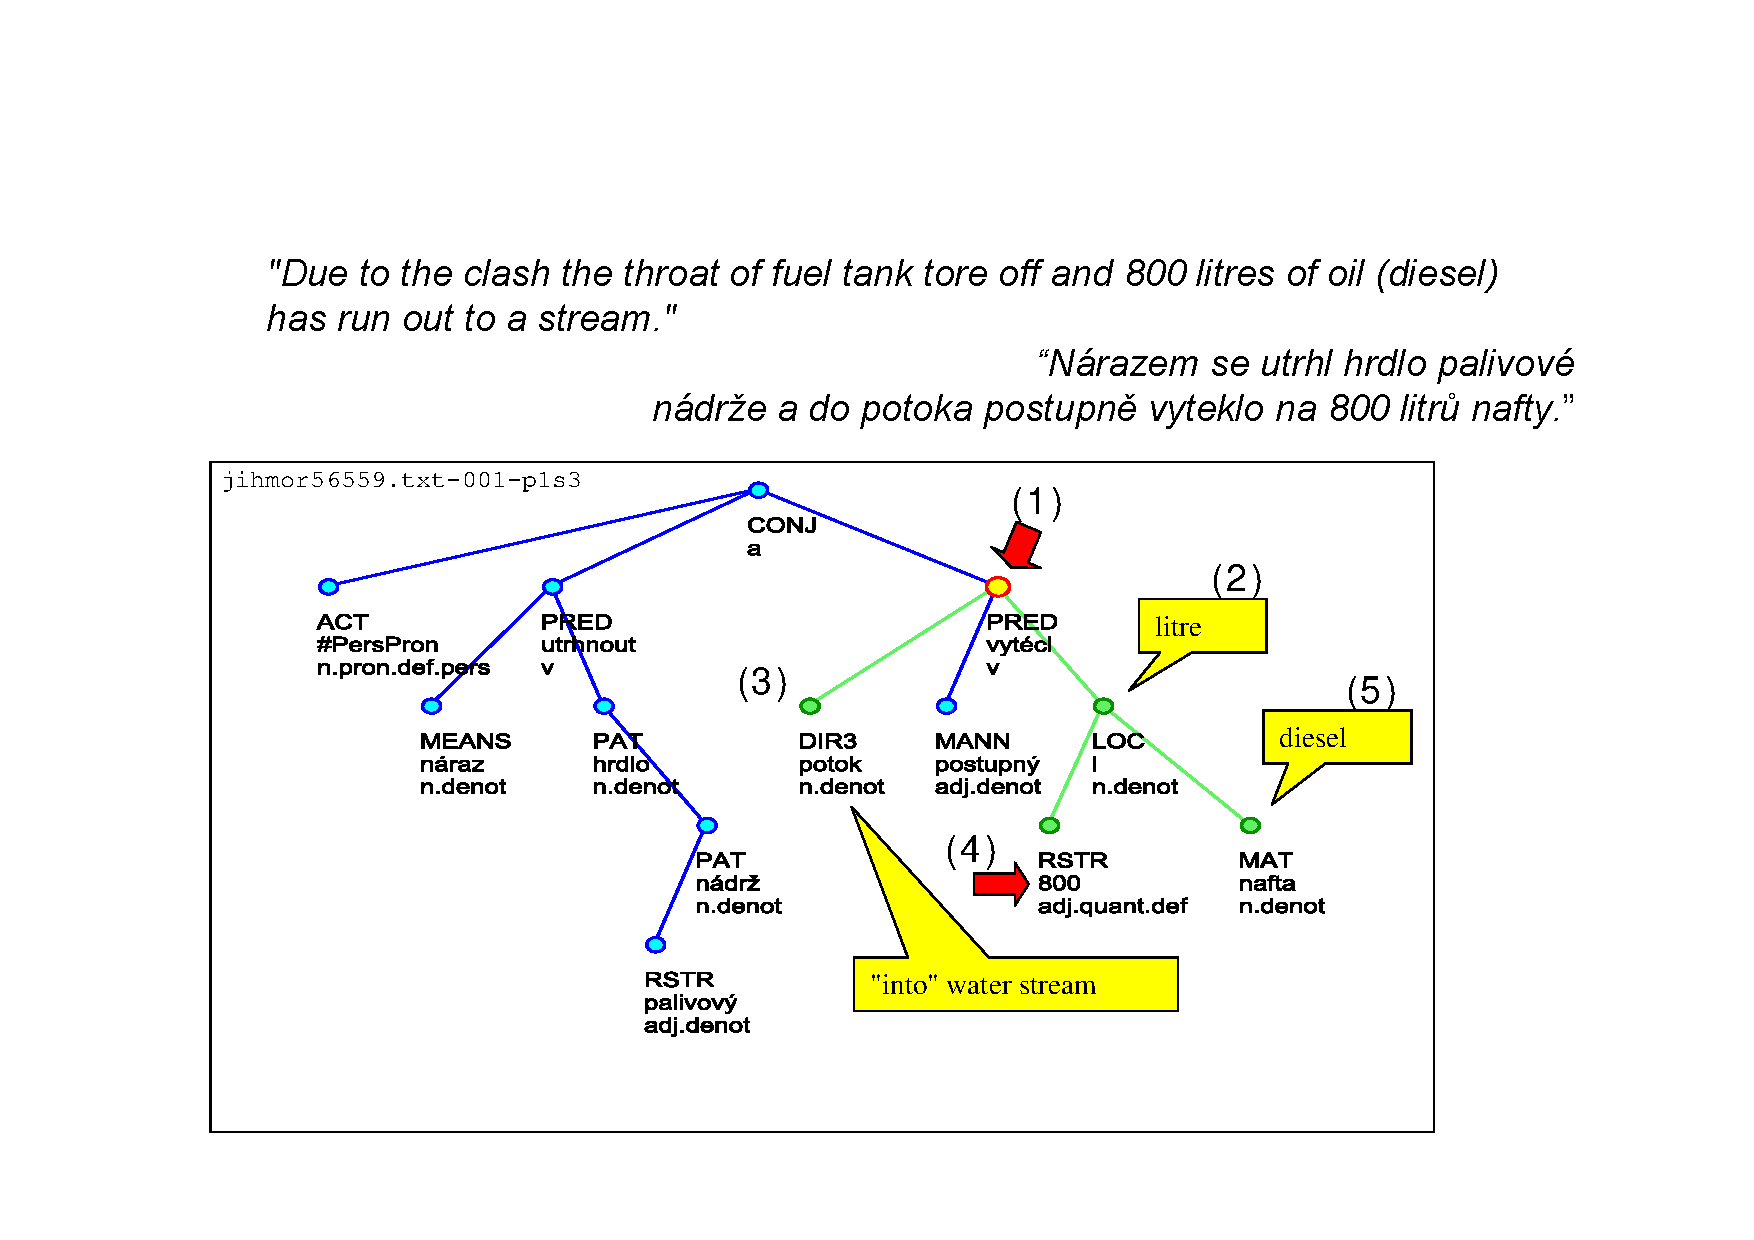
\includegraphics[height=0.8\vsize]{img/eenv_tree}}
%\end{center}
%{\scriptsize
%\textbf{SELECT} \alert{action\_type}.t\_lemma, \alert{a-negation}.m\/tag, 
%\alert{injury\_manner}.t\_lemma, \alert{participant}.t\_lemma,
%\alert{quantity}.t\_lemma \textbf{FROM} \emph{***extraction rule***} 
%}
\end{frame}


\begin{frame}{Raw data extraction output}
%\begin{center}
\centerline{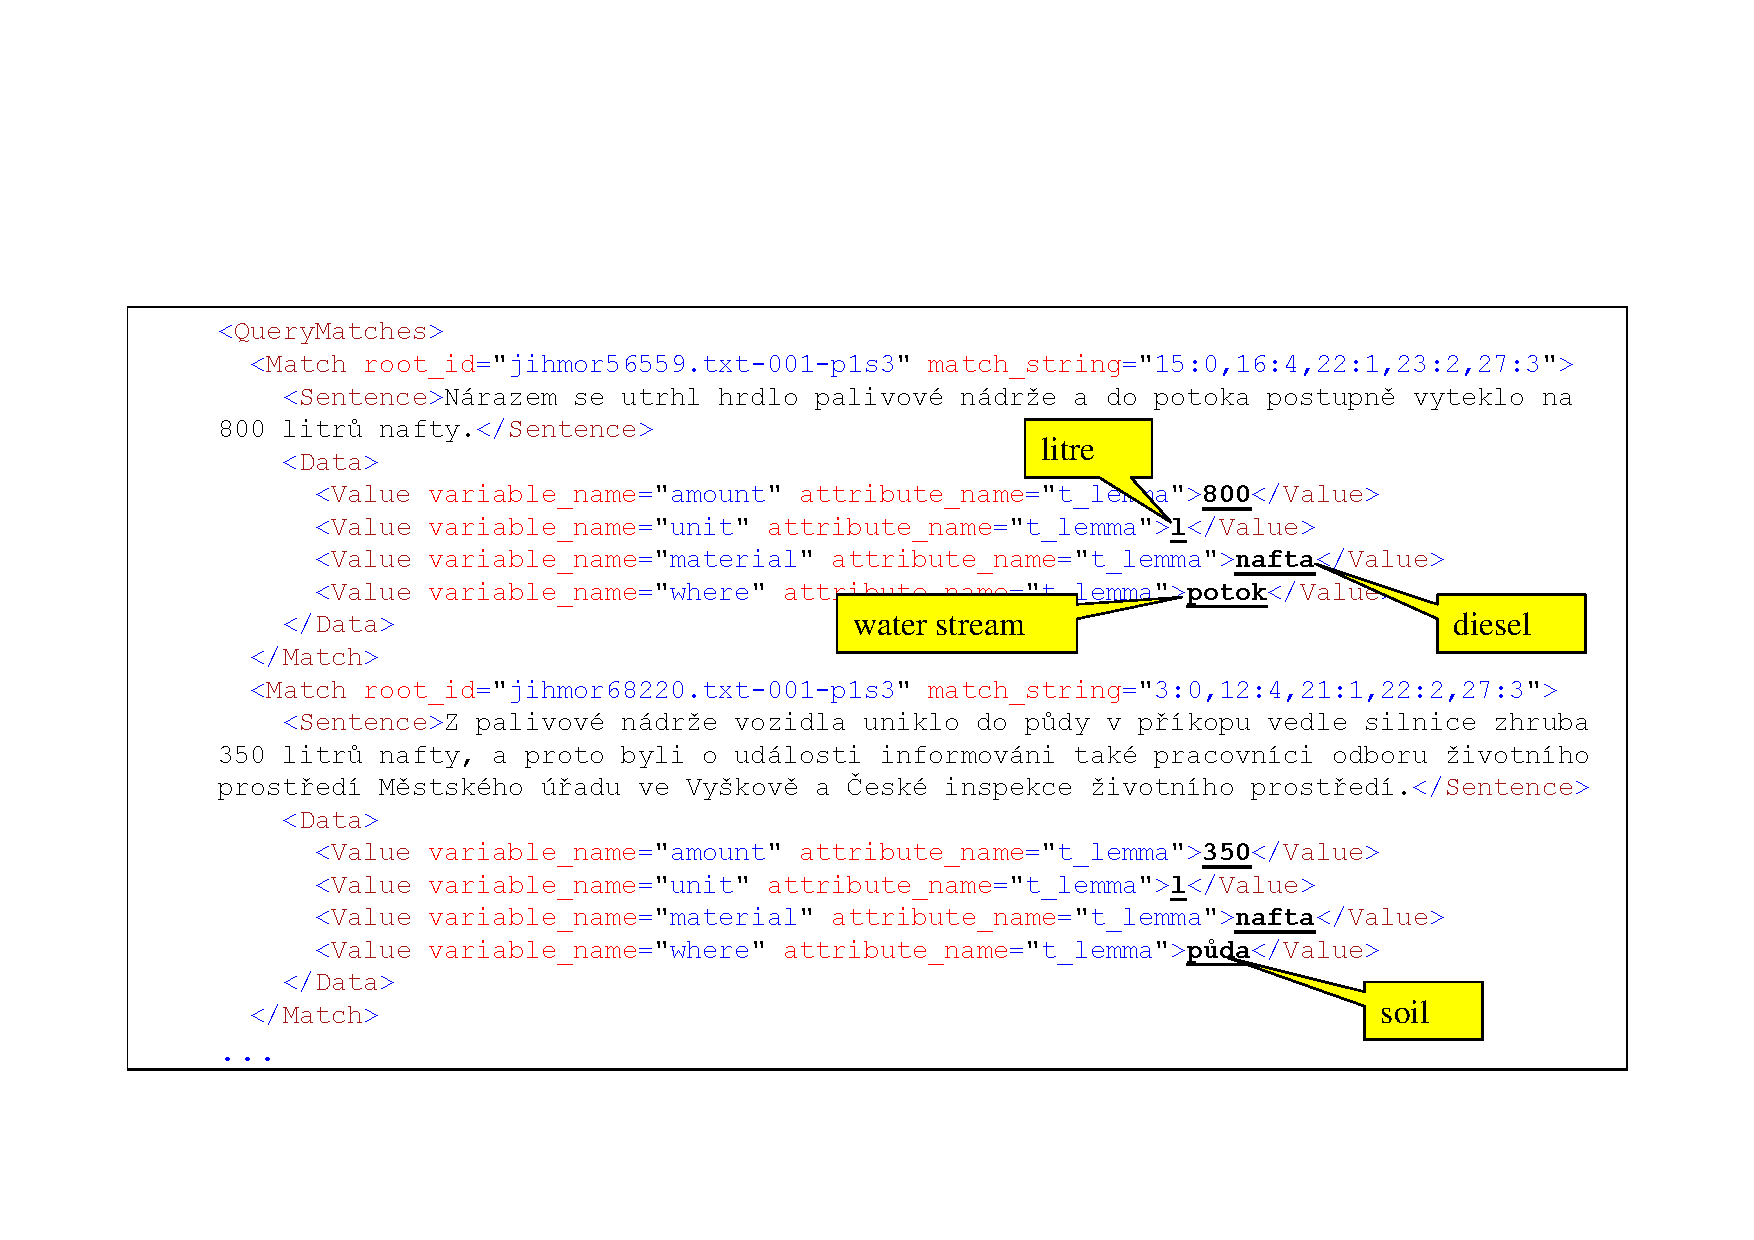
\includegraphics[height=0.77\vsize]{img/eenv_results}}
%\end{center}
{\scriptsize
\textbf{SELECT} \alert{amount}.t\_lemma, \alert{unit}.t\_lemma, 
\alert{material}.t\_lemma, \alert{where}.t\_lemma
\\ \textbf{FROM} \emph{***extraction rule***} 
}
\end{frame}



\begin{frame}{Design of extraction rules -- iterative process}
\begin{center}
\includegraphics[height=0.6\vsize]{img/DedVoj_coverge_tuning}
\end{center}
\begin{enumerate}
	\item \alert{Frequency analysis} $\rightarrow$ representative key-words.
	\item Investigating of matching trees $\rightarrow$ \alert{tuning} of tree query.
	\item \alert{Complexity} of the query $\cong$ complexity of extracted data.
\end{enumerate}
\end{frame}

\begin{frame}{Corpus of Fire-department articles}
\begin{itemize}
	\item \alert{Fire-department articles}
	\item Published by The Ministry of Interior of the Czech Republic\footnote{\url{http://www.mvcr.cz/rss/regionhzs.html}}
	\item Processed more than 800 articles 
	\\from different regions of Czech Republic
	\item 1.2 MB of textual data
	\item Linguistic tools produced 10 MB of annotations,\\run time 3.5 hours
	\item Extracting information about \alert{injured and killed people}
	\item 470 matches of the extraction rule,\\200 numeric values of quantity (described later)
\end{itemize}
\end{frame}


\subsection{Learning of Rules}
\frame{\tableofcontents[currentsubsection]}

\subsubsection{Inductive Logic Programming}

\begin{frame}{Inductive Logic Programming}
	\begin{itemize}
		\item Inductive Logic Programming (ILP) 
		\begin{itemize}
			\item is a Machine Learning procedure for \alert{multirelational} learning
			\item Heuristic and iterative method, learning is usually slow
			\item It is capable to deal with graph or \alert{tree structures} naturally 
			\item Learns form positive and negative \alert{examples}
			\begin{itemize}
				\item Positive and negative \alert{tree nodes}
				\item It is necessary to \alert{label tree nodes} from corresponding labeled text (not trivial problem)
			\end{itemize}
			\medskip
			
			\item Learned rules are strict (no weights, probabilities, etc.)			
			\begin{itemize}
				\item Easier human understanding, modification 
				\item Possibility of sharing of rules amongst different tools
				\item Lower performance (precision, recall)
			\end{itemize}
		\end{itemize}
	\end{itemize}
\end{frame}


\begin{frame}{ILP principles}
\begin{itemize}
	\item Learning examples $E=P\cup N$ (Positive and Negative)
	\item Background knowledge $B$
	\item ILP task -- to find hypothesis $H$ such that:
\end{itemize}
$$
(\forall e\in P)(B\cup H\models e) \ \ \&\  \ (\forall n\in N)(B\cup H\not\models n).
$$
%\vspace{0.5cm}
%\begin{itemize}
%	\item Fuzzy learning examples ${\mathcal E}:E\longrightarrow [0,1]$
%	\item Fuzzy background knowledge ${\mathcal B}:B\longrightarrow [0,1]$
%	\item Fuzzy ILP task -- to find hyp. ${\mathcal H}:H\longrightarrow [0,1]$ such that:
%\end{itemize}
%$$
%(\forall e_1,e_2\in E)(\forall {\mathcal M})({\mathcal M}\models_f {\mathcal B}\cup {\mathcal H}) \ :\ 
%{\mathcal E}(e_1)>{\mathcal E}(e_2)\Rightarrow \left\|e_1\right\|_{{\mathcal M}}\ge \left\|e_2\right\|_{{\mathcal M}}
%$$
\end{frame}

\begin{frame}[fragile]{ILP Example}
\begin{block}{Types of ground variables}
{\footnotesize\begin{verbatim}
animal(dog). animal(dolphin) ... animal(penguin).
class(mammal). class(fish). class(reptile). class(bird).
covering(hair). covering(none). covering(scales).
habitat(land). habitat(water). habitat(air).
\end{verbatim}}
\end{block}
\begin{block}{Background knowledge}
{\footnotesize\begin{verbatim}
has_covering(dog, hair). has_covering(crocodile, scales).
has_legs(dog,4). ... has_legs(penguin, 2). etc.
has_milk(dog). ... has_milk(platypus). etc.
homeothermic(dog). ... homeothermic(penguin). etc.
habitat(dog, land). ... habitat(penguin, water). etc.
has_eggs(platypus). ... has_eggs(eagle). etc.
has_gills(trout). ... has_gills(eel). etc.
\end{verbatim}}
\end{block}
\end{frame}

\begin{frame}[fragile]{ILP Example}
\begin{columns}
\column{.5\textwidth}
\begin{block}{Positive examples}
{\footnotesize\begin{verbatim}
class(lizard, reptile).
class(trout, fish).
class(bat, mammal).
\end{verbatim}}
\end{block}
\column{.5\textwidth}
\begin{block}{Negative examples}
{\footnotesize\begin{verbatim}
class(trout, mammal).
class(herring, mammal).
class(platypus, reptile).
\end{verbatim}}
\end{block}
\end{columns}
\bigskip
\setbeamercolor{block title}{bg=OliveGreen}
\begin{block}{Induced rules}
{\footnotesize\begin{verbatim}
class(A,reptile) :- has_covering(A,scales),
                    has_legs(A,4).
class(A,mammal) :- homeothermic(A), has_milk(A).
class(A,fish) :- has_legs(A,0), has_eggs(A).
class(A,reptile) :- has_covering(A,scales),
                    habitat(A,land).
class(A,bird) :- has_covering(A,feathers).
\end{verbatim}}
\end{block}
\end{frame}


\subsubsection{Integration of the extraction process}

\begin{frame}{Integration of ILP in our extraction process}
\begin{center}
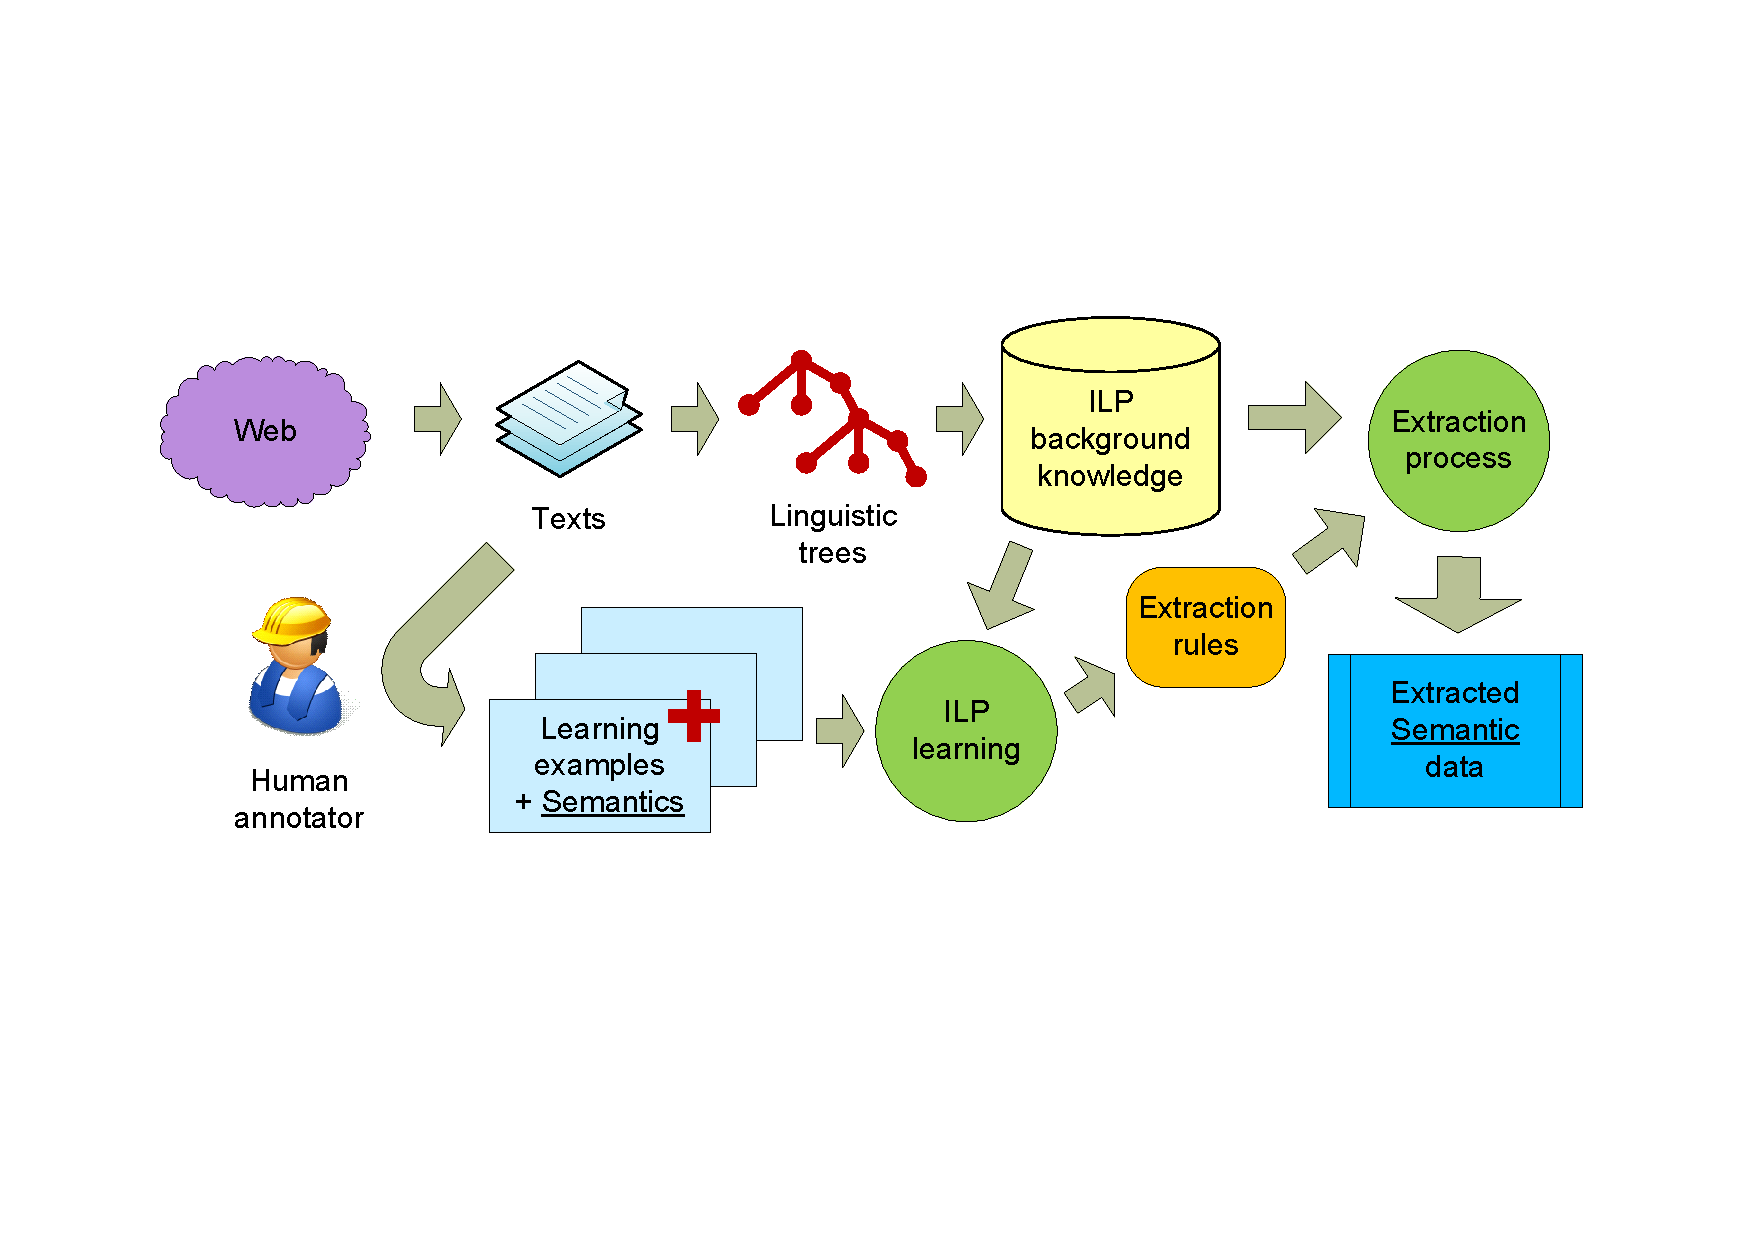
\includegraphics[width=\hsize]{img/DedVoj_ILP}
\end{center}
\begin{itemize}
	\item Main point: transformation of trees to \alert{logic representation}. 
	\item Human annotator does \alert{not} need to be a linguistic \alert{expert}.
\end{itemize}
\end{frame}

\begin{frame}{Logic representation of linguistic trees}
\begin{columns}
\column{\textwidth}
\includegraphics[height=0.9\vsize]{img/DedVoj_LogicRepresentation}
\end{columns}
\end{frame}

\begin{frame}{Root/Subtree Preprocessing/Postprocessing (Chunk learning)}
\centerline{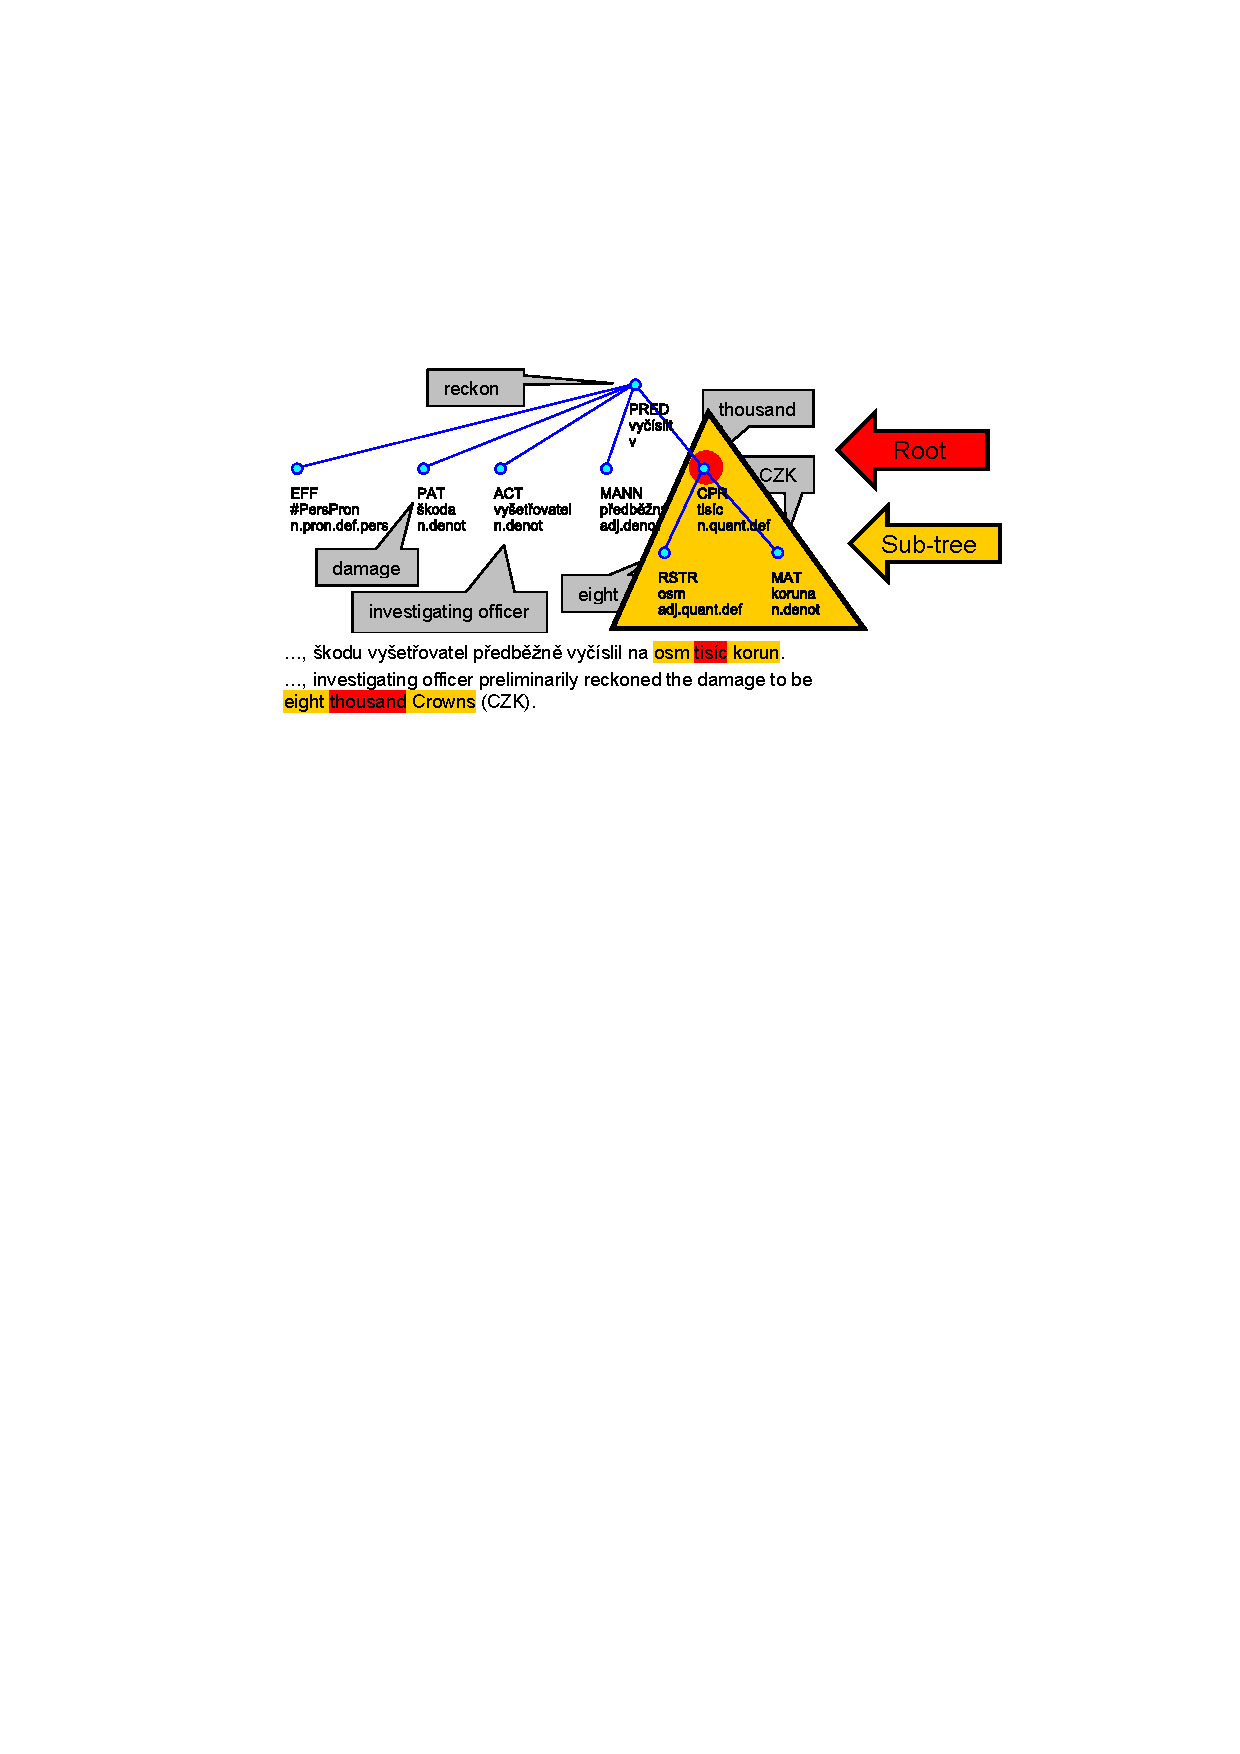
\includegraphics[width=\hsize]{img/tree-subtree}}
\end{frame}


\begin{frame}[fragile]{Examples of learned rules, Czech words are translated.}
\begin{example}
{\scriptsize


[Rule 1] [Pos cover = 14 Neg cover = 0]\\
\verb@damage_root(A) :- lex_rf(B,A), has_sempos(B,'n.quant.def'),@
\verb@   tDependency(C,B), tDependency(C,D),@ 
\verb@   has_t_lemma(D,'investigator').@ %\emph{\%vy353et345ovatel = investigator}
\smallskip

[Rule 2] [Pos cover = 13 Neg cover = 0]\\
\verb@damage_root(A) :- lex_rf(B,A), has_functor(B,'TOWH'),@
\verb@   tDependency(C,B), tDependency(C,D), has_t_lemma(D,'damage').@\\
\bigskip


[Rule 1] [Pos cover = 7 Neg cover = 0]\\
\verb@injuries(A) :- lex_rf(B,A), has_functor(B,'PAT'),@
\verb@   has_gender(B,anim), tDependency(B,C), has_t_lemma(C,'injured').@\\
\smallskip

[Rule 8] [Pos cover = 6 Neg cover = 0]\\
\verb@injuries(A) :- lex_rf(B,A), has_gender(B,anim), tDependency(C,B),@
\verb@   has_t_lemma(C,'injure'), has_negation(C,neg0).@

}
%{\tiny \begin{verbatim}
%contains_num_injured(A) :- t_lemma(A,1).
%contains_num_injured(A) :- t_lemma(A,2).
%contains_num_injured(A) :- t_lemma(A,23).
%contains_num_injured(A) :- edge(A,B), m_form(B,jeden).
%contains_num_injured(A) :- edge(A,B), m_tag(B,cn_s1__________).
%contains_num_injured(A) :- edge(B,A), functor(B,conj).
%contains_num_injured(A) :- edge(B,A), t_lemma(B,dite).
%contains_num_injured(A) :- edge(B,A), t_lemma(B,muz).
%contains_num_injured(A) :- edge(B,A), edge(B,C), m_tag14(C,1).
%contains_num_injured(A) :- edge(B,A), edge(B,C), t_lemma(C,tezky).
%contains_num_injured(A) :- edge(B,A), edge(B,C), t_lemma(C,nasledek).
%contains_num_injured(A) :- edge(A,B), edge(C,A), m_tag4(B,1), functor(C,pat).
%contains_num_injured(A) :- edge(A,B), edge(C,A), functor(C,act), a_afun(B,sb).
%contains_num_injured(A) :- edge(B,A), edge(C,B), edge(C,D), t_lemma(D,vloni).
%contains_num_injured(A) :- edge(B,A), edge(C,B), t_lemma(B,osoba), t_lemma(C,zranit).
%contains_num_injured(A) :- edge(B,A), edge(C,B), t_lemma(B,osoba), t_lemma(C,zemrit).
%contains_num_injured(A) :- edge(B,A), edge(C,B), functor(B,act), edge(C,D),
%                           a_afun(D,obj).
%contains_num_injured(A) :- edge(B,A), edge(C,B), t_lemma(B,osoba), edge(C,D), edge(D,E),
%                           functor(D,twhen).
%contains_num_injured(A) :- edge(B,A), t_lemma(A,tri), edge(B,C), edge(D,B), edge(E,D),
%                           m_tag2(C,m).
%\end{verbatim}}
\end{example}
\end{frame}



\subsection{Evaluation}
%\frame{\tableofcontents[currentsubsection]}


\begin{frame}{Evaluation results}

\centerline{
\scriptsize
\begin{tabular}{|l||r|r|r|r|r|r|r|}
\hline
\textbf{task/method} & \textbf{matching} & \textbf{missing} & \textbf{excess} & \textbf{overlap} & \textbf{prec.}\% & \textbf{recall}\% & \textbf{F1.0}\%\\
\hline
\hline
\textbf{damage/ILP} & 14 & 0 & 7 & 6 & 51.85 & 70.00 & 59.57\\
\hline
\multicolumn{5}{|l|}{\textbf{damage/ILP -- lenient measures}} & 74.07 & 100.00 & 85.11\\
\hline
\textbf{dam./ILP-roots} & 16 & 4 & 2 & 0 & 88.89 & 80.00 & 84.21\\
\hline
\textbf{damage/Paum} & 20 & 0 & 6 & 0 & 76.92 & 100.00 & 86.96\\
\hline
\hline
\textbf{injuries/ILP} & 15 & 18 & 11 & 0 & 57.69 & 45.45 & 50.85\\
\hline
\textbf{injuries/Paum} & 25 & 8 & 54 & 0 & 31.65 & 75.76 & 44.64\\
\hline
\textbf{inj./Paum-afun} & 24 & 9 & 38 & 0 & 38.71 & 72.73 & 50.53\\
\hline
\end{tabular}
}

\bigskip

\begin{itemize}
	\item 10-fold cross validation
	\item Two tasks: `damage' and `injuries'
	\item Root/subtree preprocessing/postprocessing used for `damage' task
\end{itemize}
\end{frame}


\subsection{Conclusion}

\frame{\tableofcontents[currentsubsection]}

\begin{frame}{Summary}
 \begin{itemize}
  \item Implemented a system for extraction of semantic information 
  \item Based on third party linguistic tools (\alert{TectoMT}\footnote{\url{http://ufal.mff.cuni.cz/tectomt/}})
  \item Extraction rules adopted from \alert{Netgraph}\footnote{\url{http://quest.ms.mff.cuni.cz/netgraph/}} application.
  \item \alert{ILP} used for learning rules.
  \item All methods integrated inside \alert{GATE}\footnote{\url{http://gate.ac.uk/}}.
  \bigskip
  \item Main advantages:  
	\begin{itemize}
		\item Automated selection of learning features
		\item ``Language independent''
		\item Rule based
	\end{itemize}
 \end{itemize}
\end{frame}


\begin{frame}{Future work}
 \begin{itemize}
			\item Use some \alert{Knowledge Base} (e.g. WordNet).
			\item Adaptation of this method on \alert{other languages}.
			\item Evaluation of the method on \alert{other datasets}.
			\item Be able to provide \alert{more semantics}.			
			\begin{itemize}
				\item e.g. sophisticated semantic interpretation of extracted data
			\end{itemize}
 \end{itemize}
\end{frame}
























\section{IE \& the Semantic Web}


%\section{Implementation Details}
\frame{\tableofcontents[currentsection]}

\begin{frame}{Semantic Web Introduction}
 We use semantic web \alert{ontologies} to express the semantics.
\begin{itemize}
	\item RDF, OWL languages
	\item Motivated by description logics
\medskip
	\item Concepts or \alert{Classes}
	\item Predicates or \alert{Relations} 
	\item Individuals or \alert{Instances}
\medskip
	\item RDF \alert{triples}: <Subject> <Predicate> <Object>
	\item RDF triples form a \alert{named oriented graph}	
	\begin{itemize}
		\item Basic data structure of the Semantic Web
	\end{itemize}
\end{itemize}
\end{frame}


\begin{frame}{Ontology (example)}
\centerline{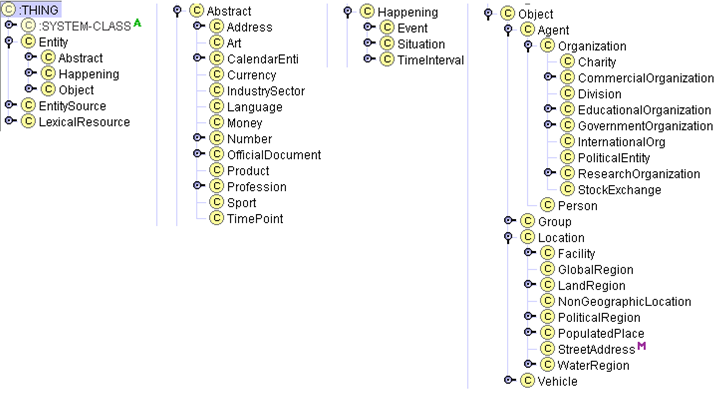
\includegraphics[width=1.1\hsize]{img/ontology}}
\begin{itemize}
	\item PROTON (PROTo ONtology) \url{http://proton.semanticweb.org/}
\end{itemize}
\end{frame}


%\subsection{Semantic Annotation}
\frame{\tableofcontents[currentsubsection]}



\begin{frame}{Semantic Annotation (\url{http://www.ontotext.com/kim/})}
\begin{columns}
\column{\textwidth}
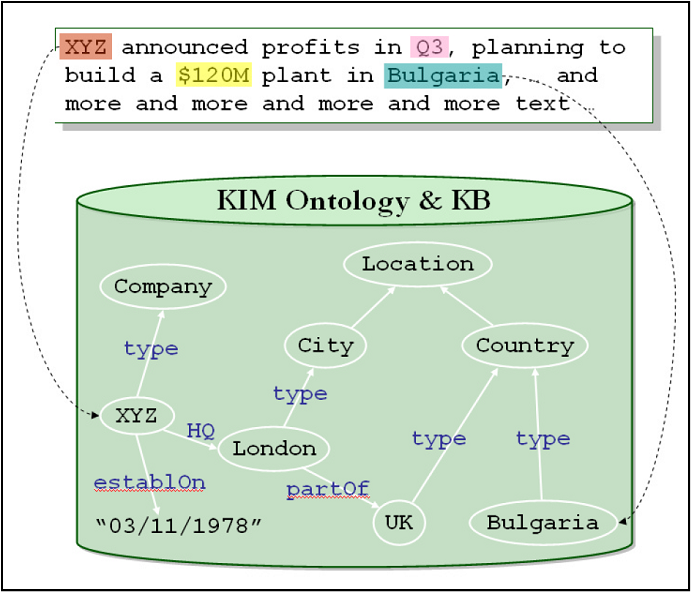
\includegraphics[height=0.9\vsize]{img/sem_annot}
\end{columns}
\end{frame}


%\subsection{Semantic Interpretation}
\frame{\tableofcontents[currentsubsection]}


\begin{frame}{Semantic interpretation of extraction rules}
\begin{center}
\includegraphics[width=\hsize]{img/DedVoj_semantic_interpretation}
\end{center}
\begin{itemize}
	\item Determines how particular values of attributes are used.
	\item Gives semantics to extraction rule.
	\item Gives semantics to extracted data.
\end{itemize}
\end{frame}

\begin{frame}{Semantic data output}
\includegraphics[width=\hsize]{img/DedVoj_instances}
\bigskip
\begin{itemize}
	\item Two instances of two ontology classes.
\end{itemize}
\end{frame}


\begin{frame}{The experimental ontology}
\begin{columns}
\column{.45\textwidth}
\includegraphics[height=0.6\vsize]{img/DedVoj_classes}
\column{.55\textwidth}
\begin{itemize}
	\item Two \alert{classes}	
		\begin{itemize}
			\item Incident and Participant
		\end{itemize}
	\item One \alert{object property} relation
		\begin{itemize}
			\item hasParticipant
		\end{itemize}
	\item Five \alert{datatype property} relations
		\begin{itemize}
			\item actionManner \\(light or heavy injury)
			\item negation
			\item actionType \\(injury or death)
			\item participantType \\(man, woman, driver, etc.)
			\item participantQuantity
		\end{itemize}
\end{itemize}
\end{columns}
\end{frame}



%\subsection{Integration with Semantic Tools}
\frame{\tableofcontents[currentsubsection]}


\begin{frame}{Transformation of PML to RDF}
\begin{itemize}
	\item Quite simple XSLT transformation
	\item Allows working with PDT annotations inside Semantic Web tools
	\begin{itemize}
		\item Ontology Editors
		\item Reasoners
		\item Query tools (graph queries)
		\item ?Visualization and navigation tools?
	\end{itemize}
	\medskip
	\item In our case interpretation of extraction rules by a OWL reasoner
\end{itemize}
\end{frame}


\begin{frame}{Extraction Rules Interpreted by OWL Reasoner}
\centerline{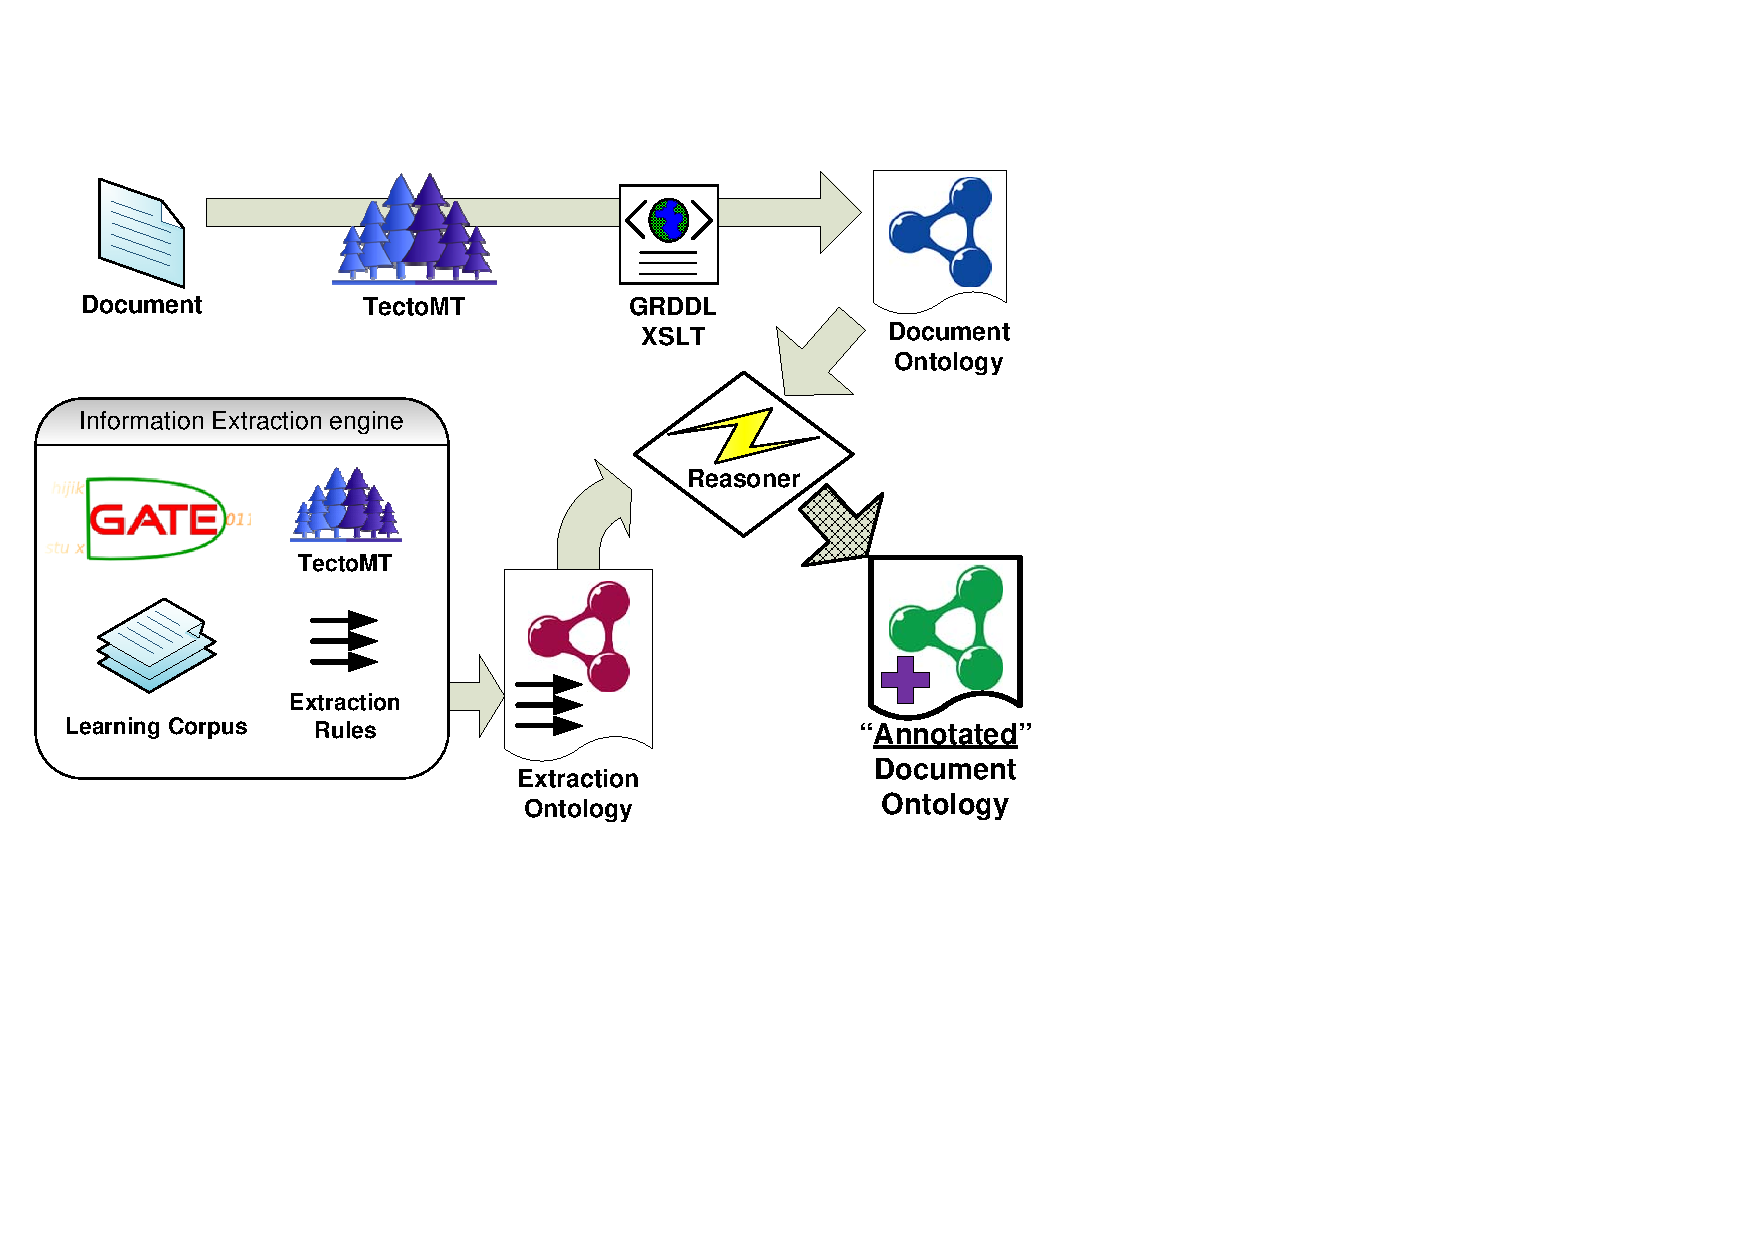
\includegraphics[width=0.9\hsize]{img/semantic_rules_app_schema}}
\begin{itemize}
	\item Tool \alert{independent} extraction ontologies
\end{itemize}
\end{frame}


\begin{frame}{PDT in The Prot�g� Ontology Editor}
\centerline{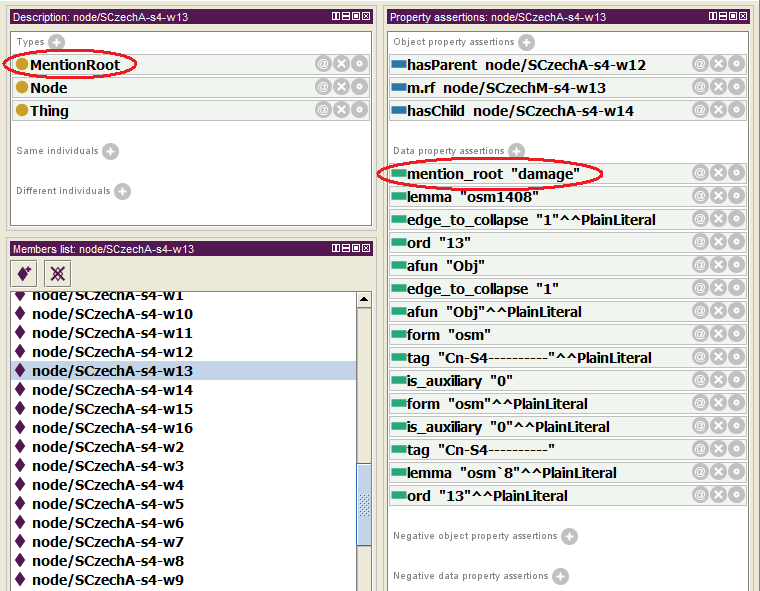
\includegraphics[width=0.9\hsize]{img/PDT_PROTEGE}}
\end{frame}

\begin{frame}[containsverbatim]
\frametitle{Examples of extraction rules in the native Prolog format.}
{\footnotesize
[Rule 1] [Pos cover = 23 Neg cover = 6]\\
\verb#mention_root(acquired,A) :-#\\
\verb#   'lex.rf'(B,A), t_lemma(B,'Inc'), tDependency(C,B),#\\
\verb#    tDependency(C,D), formeme(D,'n:in+X'), tDependency(E,C).#
\smallskip\newline
[Rule 11] [Pos cover = 25 Neg cover = 6]\\
\verb#mention_root(acquired,A) :-#\\
\verb#   'lex.rf'(B,A), t_lemma(B,'Inc'), tDependency(C,B),#\\
\verb#    formeme(C,'n:obj'), tDependency(C,D), functor(D,'APP').#
\smallskip\newline
[Rule 75] [Pos cover = 14 Neg cover = 1]\\
\verb#mention_root(acquired,A) :-#\\
\verb#   'lex.rf'(B,A), t_lemma(B,'Inc'), functor(B,'APP'),#\\
\verb#    tDependency(C,B), number(C,pl).#
}
\end{frame}

\begin{frame}[containsverbatim]
\frametitle{Examples of extraction rules in Prot\'{e}g\'{e} 4 -- Rules View's format}
{\footnotesize
[Rule 1]\\
\verb#lex.rf(?b, ?a), t_lemma(?b, "Inc"), tDependency(?c, ?b),#\\
\verb#tDependency(?c, ?d), formeme(?d, "n:in+X"),#\\
\verb#tDependency(?c, ?e)#\\
\verb#      -> mention_root(?a, "acquired")#
\smallskip\newline
[Rule 11]\\
\verb#lex.rf(?b, ?a), t_lemma(?b, "Inc"), tDependency(?c, ?b),#\\
\verb#formeme(?c, "n:obj"), tDependency(?c, ?d), functor(?d, "APP")#\\
\verb#      -> mention_root(?a, "acquired")#   
\smallskip\newline
[Rule 75]\\
\verb#lex.rf(?b, ?a), t_lemma(?b, "Inc"), functor(?b, "APP"),#\\
\verb#tDependency(?c, ?b), number(?c, "pl")#\\
\verb#      -> mention_root(?a, "acquired")#   
}
\end{frame}



\end{document}



%%% Local Variables: 
%%% mode: latex
%%% TeX-master: t
%%% End: 
